\documentclass[a4paper,twoside,openright,11pt]{book}

%
% UNSW margin guidelines:
%
%   Top >= 30mm
%   Bottom >= 20mm
%   Left >= 40mm (do they mean inner?)
%   Right >= 20mm (do they mean outer?)
%
\usepackage[
        inner=36mm, % NOPRINT
        outer=36mm, % NOPRINT
        top=30mm,
        bottom=35mm,
        headsep=10mm,
        headheight=20pt,
        footskip=12mm,
        includehead=false,
        includefoot=false,
        marginparwidth=30mm,
        heightrounded=true
        ]{geometry}

\usepackage{microtype}
\usepackage{setspace}
\onehalfspacing

\usepackage{algorithm}
\usepackage{algpseudocode}
\usepackage{graphicx}
\usepackage{amsmath}
\usepackage{amssymb}
\usepackage{mathtools}
\usepackage{listings}
\usepackage{amsthm}
\usepackage{subcaption}
\usepackage{xspace}
\usepackage{url}
\usepackage{multirow}

\title{Device Driver Synthesis}
\author{Adam Walker}

\newcommand{\buchi}{Buchi }
\newcommand{\reach}[0]{\textsc{Reach}}
\newcommand{\safe}[0]{\textsc{Safe}}
\newcommand{\concrete}[1]{#1\mathord{\downarrow}}
\newcommand{\abstractm}[1]{#1\mathord{\uparrow^m}}
\newcommand{\abstractM}[1]{#1\mathord{\uparrow^M}}
\newcommand{\forms}[0]{\mathcal{F}}
\newcommand{\vect}[1]{\vec{#1}}

\newcommand{\termite}{Termite\xspace}
\newcommand{\tsl}{TSL\xspace}

\renewcommand{\footnotesize}{\fontsize{9}{10}\selectfont}

\theoremstyle{definition}
\newtheorem*{ex}{Example}
\newcommand{\src}[1]{\texttt{\small #1}}

\lstnewenvironment{tsllisting}[1][]
{\lstset{
    escapeinside={(*@}{@*)},
    basicstyle=\footnotesize\ttfamily,
    keywordstyle=\bfseries,
    keywordstyle=\bfseries,
    sensitive=false,
    morekeywords={template, endtemplate, process, controllable, forever, wait, return, assert, goal, instance},
    identifierstyle=, 
    commentstyle=\slshape, 
    stringstyle=, showstringspaces=false,
    sensitive=false,
    morecomment=[s]{/*}{*/},
    numberstyle=\tiny,
    stepnumber=1,
    numbersep=1pt,
    emphstyle=\bfseries,
    belowskip=0pt,
    aboveskip=0pt,
    #1
}}{}


\begin{document}

\maketitle
\tableofcontents

\chapter{Introduction}

\section{Termite}
\section{Contributions}
\section{Chapter outline}

\chapter{Background}

\section{$\mu$-calculus}

\subsection{Syntax}

The $\mu$-calculus is a logic capable of expressing greatest and least solutions of fixed point equations $X = f(X)$ where $f$ is a monotone function. The set of formulas of $\mu$-calculus is defined as follows:

Let $P$ be a set of propositions, $A$ be a set of actions and $V$ be a set of variables. Then
\begin{itemize}
    \item each proposition and each variable is a formula
    \item if $\phi$ and $\psi$ are formulas then $\phi \wedge \psi$ is a formula
    \item if $\phi$ is a formula then $\neg \phi$ is a formula
    \item if $\phi$ is a formula and $a$ is and action then $[a]\phi$ is a formula
    \item if $\phi$ is a formula and $Z$ a variable then $\nu X.\phi$ is a formula provided that every free occurrence of $Z$ occurs under an even number of negations
\end{itemize}

\subsection{Semantics}

Given a labelled transition system $(S, R, V)$ where
\begin{itemize}
    \item S is a set of states
    \item $R \subseteq S \times A \times S$
    \item $V : Var \rightarrow 2^S$ maps each proposition to the set of states where the proposition is true
\end{itemize}

A $\mu$-calculus formula is interpreted as follows:
\begin{itemize}
    \item $p$ holds in the set of states $V(p)$
    \item $\phi \wedge \psi$ holds in the set of states where both $\phi$ and $\psi$ hold
    \item $\neg \phi$ holds in every state where $\phi$ does not hold 
    \item $[a]\phi$ holds in a state $s$ if every $a$-transition leading out of $s$ leads to a state where $\phi$ holds
    \item $\nu Z. \phi$ holds in any set of states $T$ such that when the variable $Z$ is set to $T$ then $\phi$ holds for all of $T$. It is the greatest fixpoint of $\phi$.
\end{itemize}

\section{Two player games}

Two-player games are a useful formalism for reactive synthesis. Many problems in electronic design automation, industrial automation and robotics can be formalised as a game. In particular, the driver synthesis problem can be formalised as a game, and, this is the formalism around which Termite is built. Here, we present the fundamentals of $\omega$ regular games. 

\subsection{Formalism}

A two player game is played by player~1 against its opponent, player~2. It consists of a possible infinite state space $S$ on which the game is played. The game is always in some state $s \in S$ called the current state. The game progresses from state to state according to a transition relation, $\delta \subseteq S \times L \times S$ where $S$ is the set of states and $L$ is a set of label variables. A transition $t \in S \times L \times S$ is allowed in the game iff $t \in delta$. 

The meaning of the label $l \in L$ depends on the type of game, but for now we will consider turn based games. In a turn based game, $S$ is partitioned into two sets: the player~1 set $\tau_1$ and the player~2 set $\tau_2$, where $\tau_1 \cap \tau_2 = \emptyset$ and $ \tau_1 \cup \tau_2 = S$. When $s \in \tau_1$ player 1 gets to pick $l$ and when $s \in \tau_2$ player 2 gets to pick $l$.

Lastly, each game has an associated set of initial states $I \in 2^S$ where execution of the game begins.

Putting this all together, we can identify a \emph{turn based game structure} $G = \langle S,L,I,\tau_1,\tau_2,\delta \rangle$ with a turn based game.

A game proceeds in an infinite sequence of rounds, starting from some initial state. The infinite sequence of states visited $(s_0, s_1,\ldots) \in S^\omega$ is called a path. 

A game is won by player 1 if, by picking suitable labels, they can force the path to be within a winning set of state objectives $\Phi \subseteq S^\omega$, where $S^\Omega$ is the set of all infinite sequences of states in $S$. An arbitrary set of infinite sequences is an extremely general, but not practically useful, way of defining an objective. In the following sections we will consider some more restricted objectives that have practical uses.

\subsection{Safety and reachability games}

The two simplest objectives are safety and reachability. A safety objective is defined by a set $SAFE \subseteq S$ that player 1 must force the game to stay within, regardless of the labels that player 2 picks. Formally, a run is safe if $\forall i. s_i \in SAFE$. 

The dual of a safety objective is a reachability objective. A reachability objective is defined by a set $REACH \subseteq S$ that player 1 must force the game to visit at least once, regardless of the labels that player 2 picks. Formally, a reachability run is winning if $\exists i. s_i \in REACH$

\subsection{Strategies, counterexamples}

Given an objective, a game is either winning for player~1 or it is losing. If it is winning, then there exists a strategy for player~1. Informally, a strategy tells player~1, in any state, which label it must play and ensures that if player~1 adheres to the strategy then the objective will be satisfied.

Formally, a strategy for player~1 is a function $\pi_1 : S^* \times \tau_1 \rightarrow L$ that, in any player~1 state, associates the history of the game with a label to play. It is known that for complete information games, as we are considering, if there exists a strategy, then there also exists one that only depends on the current state. Thus, we can simplify the definition of a strategy for player~1 to be a function $\pi_1 : \tau_1 \rightarrow L$ that only depends on the current state.

Conversely, if the game is losing for player~1, then there exists a spoiling strategy for player~2, that is, a strategy for player~2 that ensures that, no matter which labels player~1 picks, there is no way that player~1 can satisfy its objective.

Formally, a counterexample strategy for player~1 is a strategy for player~2 which is a function $\pi_2 : \tau_2 \rightarrow L$ that associates any player~2 state with a label for player~2 to play. Again, we have simplified the definition as there must exist a strategy that only depends on the current state. 

\subsection{Buchi, fairness and GR(1) games}
Here we consider objectives that are more complex and more useful in practice.

\paragraph{Buchi}
A Buchi objective is defined by a set $BUCHI \subseteq S$ that player~1 must always be able to force execution of the game into. This differs from a reachability game in that the region must always be reachable, not just once. When it has been reached once, it must be reachable again, and so on. So, it must be reachable infinitely many times. Formally, a run is buchi winning if $\forall i. \exists j>i. s_j \in BUCHI$

\paragraph{Generalized Buchi}
A Generalized Buchi objective is defined by a set of sets $BUCHIS \subseteq 2^S$. Player~1 must always be able to force execution into each set $BUCHI \in BUCHIS$. Formally, a run satisfies a generalized Buchi objective if $\forall i. \forall BUCHI \in BUCHIS. \exists j>i. s_j \in BUCHI$.

\paragraph{Fairness}
Sometimes it is necessary to rule out invalid plays that are not easily ruled out by changing the state machine. For this we use fairness conditions. A fairness condition is a set of states which we may assume that all valid runs of the game eventually leave. If a spoiling strategy exists that results in an unfair run, it does not count. Formally, a run satisfies a fair reachability objective if $\forall i. \exists j>i. s_j \notin UNFAIR \rightarrow \exists i. s_i \in REACH$. 

\paragraph{GR(1)}
A Generalized Reactive 1, or GR(1) objective, is a generalized Buchi objective with multiple fairness conditions. In practice, this turns out to be a very useful type of objective. Formally, a run satisfies a GR(1) objective if $\forall i. \forall UNFAIR \in UNFAIRS \exists j>i. s_j \notin UNFAIR \rightarrow \forall i. \forall BUCHI \in BUCHIS. \exists j>i. s_j \in BUCHI$.

\subsection{Solving games}
\subsubsection{Controllable predecessor}

All of the synthesis algorithms for games I will be describing use a function called the controllable predecessor (abbreviated CPre). CPre is a function from a set of game states ($2^S$) to another set of game states. Given a set $T$, $CPre(T)$ returns the set of states from which player 1 can force execution into $T$ in one step. 

The exact details of $CPre$ do not matter and it can be considered to be a parameter to the game solving algorithms. The function it computes depends on the application and I will be describing the driver synthesis $CPre$ later. For now, the only property of $CPre$ that we require is that it is monotonic, ie. if $X \subseteq Y$ then $CPre(X) \subseteq CPre(Y)$. Clearly, any reasonable $CPre$ function will have this property.

\subsubsection{Safety and reachability}

We will start with reachability as it is the easiest to understand. A state is winning in a reachability game if there is some finite $i$ such that we can guarantee that after $i$ rounds of the game, execution will have, at least once, entered a state in $REACH$.

We can define the winning region inductively. It is obviously possible to reach the set $REACH$ from $REACH$ in 0 steps as we are already there. This is the base case. It is also possible to reach $REACH$ from $x \in S$ in $N + 1$ steps or fewer iff it is possible to reach $REACH$ from all of $Y \subseteq 2^S$ in $N$ steps or fewer and $x \in CPRE(Y)$.

This suggests an algorithm. We start with $REACH$, apply $CPRE$ to get the states winning in 1 step, combine with $REACH$ again to get the states reachable in 1 step or less, and then repeat. On each iteration we find the states winning in $N$ or less steps. Two questions remain: 

\begin{itemize}
    \item An algorithm must terminate, so, when should we stop iterating?
    \item After termination, has the algorithm found all the winning states?
\end{itemize}

Observe that $W_{N+1} \supseteq W_N$. So, on each iteration, we either grow the winning set or it remains the same. Also observe that our set $S$ is finite, which means that $2^S$ is also finite. As set inclusion is a transitive relation, we cannot grow our winning set forever, so eventually we must reach a fixed point of the CPRE function. 

%TODO: $CPRE$ isnt the order preserving function
Or, if you prefer, the power set of $S$ can be ordered by set inclusion to obtain a complete lattice with supremum $S$ and infimum $\emptyset$. $CPRE$ is an order preserving function, so by the Knaster-Tarski theorem the set of fixed points of $CPRE$ is also a complete lattice. Thus there exists a greatest and least fixed point (as the lattice is complete). The least fixed point of $CPRE$ is clearly obtained by iteration starting from the least element of the lattice, ie. $\emptyset$.

Thus, we will eventually reach a fixed point, and, this is when we should stop iterating as further iterations will not change the winning set. Furthermore, we know that after any finite number $N$ of iterations where $N$ is greater than the number of iterations required to reach the fixed point, the winning region will remain $WIN$. Thus $WIN_N = WIN$ and we have found all winning states.

Safety games are the dual of reachability games and are also solved by iterating the controllable predecessor. They will not be described here.

\begin{equation}
REACH(T) = \mu X. CPre(X \vee T)
\label{equ:mu_reach}
\end{equation}

\begin{equation}
SAFE(T) = \nu X. CPre(X \wedge T)
\label{equ:mu_safe}
\end{equation}

\begin{algorithm}[t]
\begin{algorithmic}
\Function{Reach}{$REACH$}
\State $Y \gets \varnothing$
\Loop
\State $Y' \gets CPre(Y \cup REACH)$
\If {$Y' = Y$} 
\State\Return $Y$\EndIf
\State $Y \gets Y'$
\EndLoop
\EndFunction
\end{algorithmic}
\caption{Solving a reachability game}
\label{a:reach}
\end{algorithm}

\begin{algorithm}[t]
\begin{algorithmic}
\Function{Safe}{$SAFE$, $CPre$}
\State $Y \gets S$
\Loop
\State $Y' \gets CPre(Y \cap SAFE)$
\If {$Y' = Y$} 
\State\Return $Y$\EndIf
\State $Y \gets Y'$
\EndLoop
\EndFunction
\end{algorithmic}
\caption{Solving a safety game}
\label{a:safe}
\end{algorithm}

\subsubsection{Buchi}

To solve a Buchi game, you first find the set from which you can reach the goal once as you do for a reachability game. Then, you use this set to find the set from which you can reach the goal twice, three times, and so on until you get to another fixed point. 

Imagine you have solved the reachability game $R = REACH(T)$ where $T$ is the Buchi target set and $R$ is the winning region. Then $V = R \wedge T$ is a subset of the goal from which you can reach the goal one more time. Computing $W = REACH(V)$ gets you the set of states from which you can reach the goal twice. Iterating this procedure will eventually lead to a fixed point as $REACH$ is a monotonic function.

This fixed point is the set of states from which you can reach the goal any number of times. Thus, it is the winning set of the Buchi game. The algorithm is given in algorithm \ref{a:buch}.

\begin{algorithm}[t]
\begin{algorithmic}
\Function{Buchi}{$T$, $CPre$}
\State $Y \gets S$
\Loop
\State $Y' \gets \Call{Reach}{Y \cap T}$
\If {$Y' = Y$} 
\State\Return $Y$\EndIf
\State $Y \gets Y'$
\EndLoop
\EndFunction
\end{algorithmic}
\caption{Solving a \buchi game}
\label{a:buchi}
\end{algorithm}

\begin{equation}
BUCHI(T) = \nu X. \mu Y. CPre(Y \vee (X \wedge T))
\label{eqn:mu_buchi}
\end{equation}

\subsubsection{Generalized Buchi}

Solving a generalized buchi game is similar to a buchi game except that you find the set from which you can reach any goal once, then any goal twice, etc. The algorithm is a small modification to the buchi algorithm and is given in algorithm \ref{alg:gen_buchi}.

\begin{algorithm}[t]
\begin{algorithmic}
\Function{Generalized\_Buchi}{$T$, $CPre$}
\State $Y \gets S$
\Loop
\State $Y' \gets S$

\For{\textbf{each} G in Goals}
\State $Y' \gets Y' \wedge \Call{Reach}{Y \cap G}$
\EndFor

\If {$Y' = Y$} 
\State\Return $Y$\EndIf
\State $Y \gets Y'$

\EndLoop
\EndFunction
\end{algorithmic}
\caption{Solving a generalized \buchi game}
\label{alg:gen_buchi}
\end{algorithm}

\begin{equation}
    GEN\_BUCHI(T) = \nu X. \prod_{G \in GOALS} \mu Y. CPre(Y \vee (X \wedge G))
\label{eqn:mu_buchi}
\end{equation}

\subsubsection{GR(1)}

Next, we need to add fairness. Consider a fair reachability game. An unfair region is a region that we can assume execution will leave, regardless of the loops it contains. We modify the controllable predecessor to create a fair controllable predecessor that takes this into account. Intuitively, the algorithm considers a block of unfair states to be winning if the only way out leads to an already winning state. To achieve this, we play a variation of a safety game where we can win if we stay entirely within the unfair set or upon exiting the unfair set we are immediately in the target set $T$. The procedure for the fair controllable predecessor is given in algorithm \ref{a:fair_cpre}. Using $Fair\_CPre$ as the $CPre$ operator in the reachability algorithm (algorithm \ref{a:reach}) yields the fair reachability algorithm. The reader is invited to check that this algorithm correctly determines that all states in figure \ref{fig:fair} are winning.

\begin{algorithm}[t]
\begin{algorithmic}
\Function{Fair\_CPre}{$CPre$, $T$}
\State $Y \gets S$
\Loop
\State $Y' \gets \Call{CPre}{Y \cap T}$
\If {$Y' = Y$} 
\State\Return $Y$\EndIf
\State $Y \gets Y'$
\EndLoop
\EndFunction
\end{algorithmic}
\caption{The fair controllable predecessor}
\label{a:fair_cpre}
\end{algorithm}

\begin{equation}
FAIR\_CPRE(U, T) = \nu X. CPre((U \wedge X) \vee T)
\label{eqn:mu_fair}
\end{equation}

Finally, if we combine the Buchi game with the fair controllable predecessor we get a GR(1) game. The procedure is given in algorithm \ref{a:gr1}.

\begin{algorithm}[t]
\begin{algorithmic}
\Function{GR(1)}{$CPre$, $T$}
\State\Return \Call{Buchi}{$T$, Fair\_Cpre(CPre)}
\EndFunction
\end{algorithmic}
\caption{GR(1) game}
\label{a:gr1}
\end{algorithm}

\begin{equation}
GR1(G, U) = \nu X. \mu Y. \nu Z. CPre((U \wedge Z) \vee (G \wedge X) \vee Y)
\label{equ:mu_gr1}
\end{equation}

\subsection{Extracting strategies}

\subsubsection{Reachability}

Once we have solved a game and determined that it is winning, we can extract a strategy. In driver synthesis, the strategy is used to generate the driver. A strategy is a relation between states and labels to play that are guaranteed to get you closer to the goal. Strategy extraction requires a straightforward modification to the game solving algorithm.

When extracting a strategy for a reachability game we need to record, for each iteration, how we got one step closer to the goal. The algorithm is given in algorithm \ref{alg:reach_strat}. 

The strategy relation is initialized to the empty set. Then, we perform an iteration of the controllable predecessor. This time we use \textsc{CPre\_Strat}, which, in addition to computing the next reachable set, also computes a relation between the newly discovered winning states and the labels that take execution from these newly discovered states one step closer to the goal.

On each iteration we combine this strategy for the newly discovered states with the strategy for the previously discovered states until we reach a fixed point as before. In the end, the strategy relates each state in the final winning region to a label that takes the game one step closer to the goal.

\begin{algorithm}[t]
\begin{algorithmic}
\Function{Reach\_Strat}{$REACH$}
\State $Y \gets \varnothing$
\State $STRAT \gets \varnothing$
\Loop
\State $(Y', STRAT') \gets CPre\_Strat(Y \cup REACH)$
\If {$Y' = Y$} 
\State\Return $(Y, STRAT)$\EndIf
\State $STRAT \gets STRAT \cup STRAT'$
\State $Y \gets Y'$
\EndLoop
\EndFunction
\end{algorithmic}
\caption{Extracting a strategy for a reachability game}
\label{alg:reach_strat}
\end{algorithm}

\subsubsection{Buchi}

Like a reachability strategy, a strategy for a buchi game must ensure that we eventually get to the goal. However, it must also ensure that once we get to the goal it is still possible to reach the goal again. 

A buchi strategy must guarantee that we can reach the intersection of the goal and the winning region, which will be non-empty if the game is winnable. The algorithm for computing the strategy in a buchi game is given in algorithm \ref{alg:buchi_strat}.

\begin{algorithm}[t]
\begin{algorithmic}
\Function{Buchi\_Strat}{$REACH$}
\State $win \gets \Call{Buchi}{REACH}$
\State \Return \Call{Reach\_Strat}{$win \cap REACH$}
\EndFunction
\end{algorithmic}
\caption{Extracting a strategy for a buchi game}
\label{alg:buchi_strat}
\end{algorithm}

\subsubsection{Generalized buchi}

Like a generalized buchi strategy must ensure that we can always get to any of the goals. A generalized buchi strategy must guarantee that we can reach the intersection of any of the goals and the winning region, which will be non-empty if the game is winnable. The algorithm for computing the strategy in a generalized buchi game is given in algorithm \ref{alg:gen_buchi_strat}. It returns one strategy for each goal that ensures you can get to the goal while remaining in the winning region. 

\begin{algorithm}[t]
\begin{algorithmic}
\Function{Gen\_Buchi\_Strat}{$REACH$}
\State $win \gets \Call{Generalized\_Buchi}{REACH}$

\For{\textbf{each} G in Goals}
\State \Return \Call{Reach\_Strat}{$win \cap G$}
\EndFor

\EndFunction
\end{algorithmic}
\caption{Extracting a strategy for a generalized buchi game}
\label{alg:gen_buchi_strat}
\end{algorithm}

\subsubsection{Fair reachability}

A strategy for a fair reachability game must ensure that we can reach the goal assuming that an unfair condition is not forever true. Conceptually, it tries to keep execution within an unfair region for which the only way out takes us a step closer to the goal. The algorithm for computing the strategy in a fair reachability game is given in algorithm \ref{alg:fair_reach_strat}.

\subsubsection{GR(1)}

\subsection{Extracting counterexamples}

\section{Symbolic games}

The algorithm described so far appears very inefficient. Consider a reachability game. We are performing a backwards breadth-first search starting from $REACH$. If we were to implement it directly as described, we would need a set abstract datatype to represent the winning set. Some of the games we have solved with Termite have upwards of $2^{80}$ states, even after abstraction. Clearly, explicitly representing the winning set will never succeed. 

Identical problems are encountered in model checking. The breakthrough that revolutionised model checking was to represent state sets implicitly as a characteristic equation over state variables.

\subsection{State variable encoding}

Symbolic games are defined over a finite set of state variables, $X$, and a finite set of label variables $Y$. We redefine $S$, the set of states, to be the set of possible valuations of each state variable in $X$. That is, each state $s \in S$ is given by a valuation of all of the state variables in $X$. Similarly, we redefine $L$, the set of labels, to be the set of possible valuations of each label variable in $Y$.

For a set $Z$ of variables, we denote by $\forms(Z)$ the set of propositional formulas constructed from the variables in $Z$. The characteristic formula of a set of states $T$ is a function $f \in \forms(X)$ that evaluates to true for the valuation corresponding to a state $s \in T$ and false otherwise. We use characteristic formulas to represent sets of states as it is more compact than explicitly listing each member of the set. This is called a symbolic representation.

Likewise, $\delta$ is specified by a formula in $\forms(X \bigcup Y \bigcup X')$, where $X' = \{x' \mid x \in X \}$ is the set of next state variables.

\subsection{Symbolic algorithms}

We can redefine Algorithms 1-4 using characteristic functions instead of explicit sets. The algorithms are superficially similar except they use conjunction and disjunction to modify sets instead of explicit set intersection and union. TODO: should I show the algorithms again with symbolicness?

\subsection{Strategy generation}
\subsection{Binary decision diagrams}

A binary decision diagram is an efficient data structure for manipulating large propositional formulas. 

\subsubsection{Binary decision trees}

\begin{figure}[t]
\centering
\includegraphics[width=0.5\linewidth]{diagrams/decistree.pdf}
\caption{A binary decision tree for $x \vee y$}
\label{fig:decis_tree}
\end{figure}

Figure \ref{fig:decis_tree} shows a decision tree for the disjunction of two variables. The root node represents the disjunction function. The child nodes, or internal nodes, represent variables and the leaf nodes, or terminal nodes represent the outcome of the function. Terminal nodes are labelled either True or False. Given a valuation of X and Y, we can evaluate the function by starting at the root and taking the solid edge if the variable represented by the node is assigned to True in the valuation and taking the dashed edge if the value is assigned to False. 

For example, in figure \ref{fig:decis_tree}, for the valuation $x=True$ and $y=False$, we start at the root node which is labelled x as x is this node's decision variable. X is assigned to True so we follow the solid edge to the next decision node which is labelled y. Y is assigned to false so we take the dashed edge and arrive at a terminal node whos value is 1, meaning that the function evaluates to 1 for this variable valuation.

\subsubsection{Ordered binary decision trees}

If the order in which the variables appear along all paths starting from the root node and ending at a terminal node are the same, then the decision tree is called an ordered decision tree. The decision tree in figure \ref{fig:decis_tree} is ordered.

\subsubsection{Reduced ordered binary decision diagrams}

\begin{figure}[t]
\centering
\includegraphics[width=0.5\linewidth]{diagrams/bdd.pdf}
\caption{A binary decision diagram}
\label{fig:bdd}
\end{figure}

A reduced ordered binary decision diagram (from now on, just BDD) is created by sharing subtrees as much as possible within an ordered binary decision tree.

In particular: 
\begin{itemize}
    \item Terminal nodes with the same label are merged. This means there are only two terminal nodes: True and False.
    \item Internal nodes with the same children are merged.
    \item Nodes with two identical children are removed and all incoming nodes are redirected to the child.
\end{itemize}

Figure \ref{fig:bdd} is an example of a BDD.

\subsubsection{Complement arcs}

\subsubsection{Canonicity}
Given a variable ordering, reduced ordered binary decision diagrams are a canonical representation of a function. This means that given a function $f$ of some set $S$ of variables, another function $g$ that evaluates to the same value for each valuation of the variables in $S$ will be represented by exactly the same BDD.

In practice, one uses a BDD library such as CUDD \cite{cudd} to build and manipulate BDDs. CUDD keeps track of all BDDs and subtrees within the BDDs that have been created and reuses these to ensure that all BDDs remain in reduced form. This, along with canonicity, means that BDD equivalence can be checked in constant time simply by checking pointer equality of the two BDDs.

\subsubsection{Conjunction and disjunction}

BDDs are not usually built as decision trees and then reduced. Instead, they are build from the bottom up, starting with the terminal and variable nodes and combining these using conjunction, disjunction and negation.

Conjunction and disjunction are computed using a straightforward recursive algorithm that wont be given here, but if the reader is interested, more information can be found in \cite{somenzi_bdd}. An important result is that, in the worst case, the procedure runs in time proportional to the product of the sizes of the two input BDDs. Furthermore, the size of the resulting BDD may be equal to the product of the sizes of the two input BDDs in the worst case. A strength of BDDs, however, is that this worst case rarely happens in practice. 

\subsubsection{Function composition and quantification}

Function composition is where a BDD representing some function is substituted for a variable in another BDD.

Given a function $f(x_1,\cdots,x_n)$, we define existential quantification of $f$ with respect to $x_i$ as $\exists x_i. f = f_{x_i} \vee f_{x_i}$ and universal quantification of $f$ with respect to $x_i$ as $\forall x_i. f = f_{x_i} \wedge f_{x_i}$.

Quantifications of the same type commute, so quantification with respect to a set of variables is well defined. 

\subsubsection{Variable ordering}

The number of nodes in a BDD depends drastically on the ordering chosen for the variables. Therefore, the space occupied by the BDDs and the time spent performing operations on them also depends on the variable ordering. This directly affects the performance of game solving algorithms that use BDDs as the symbolic data structure. 

Optimal variable orderings may be found using exact algorithms, but these are prohibitively expensive for BDDs with more than a few nodes. In practice heuristics are used which produce good, but not optimal orderings. One such heuristic is Ruddell's sifting algorithm \cite{sifting}.

The CUDD BDD package performs \emph{dynamic variable ordering}, which means that once the number of BDD nodes the package knows about grows past a certain threshold, the package automatically performs the requested reordering algorithm on all BDDs that exist in the manager. Dynamic variable ordering is critical to the performance of game solving algorithms that utilise BDDs and therefore we always enable it.

\chapter{Driver synthesis as a Game}

\section{Scope}
What goes here?

\section{Formalism}

\subsection{Concurrent games}

Our game formalism for termite makes use of concurrent games. Concurrent games differ from simpler turn based games in that in each state both players get to pick a label and the next state that the game transitions to is some function of both of those labels. Turn based games are a special case of concurrent games where in player~i states the next state is entirely determined by the label played by player~i and the other player's label is ignored. 

It is important to specify which player gets to pick their label first and if the second player gets to have knowledge of the label that the first player picks when choosing their label. In Termite, player~1 (the driver) has to pick first and the environment (device and operating system) gets to pick second with knowledge of the label that the driver picked. This makes the game more difficult to win for the driver.

We call the part of the label that the driver gets to pick $C$ (for controllable) and the part that the environment gets to pick $U$ (for uncontrollable). Our transition relation is defined over the current state $S$, as well as the label $C$ and $U$. Our controllable predecessor becomes:

\begin{equation}
    CPre(X) = \exists C. \forall U. \forall N. TRANS(S, C, U) \rightarrow X'
\end{equation}

We define a special variable that is part of the environment's label called \textsc{Turn}.

\subsection{Device and OS state machines and synchronization}

\subsection{GR(1) based formalism}

As a concrete example, we could create a crude formalism for driver synthesis using only a reachability game. Consider, for example, figure \ref{fig:reach}, which shows the state machine for a game to control a hypothetical network controller. Solid lines indicate controllable transitions and dashed lines indicate uncontrollable transitions. Execution begins in the leftmost state where the OS may initiate a network transfer by choosing the `send' label. The goal of the game is the rightmost state (labelled `G') as this is the point where player 1 has completed the request. So, to win, player 1 (who controls the transitions with solid lines) must ensure that execution of the state machine reaches the goal. 

\begin{figure}[t]
\centering
\includegraphics{diagrams/reachgame.pdf}
\caption{Reachability game for simple network device}
\label{fig:reach}
\end{figure}

The network device has two 8-bit registers, command (abbreviated cmd) and data. Writing 0x01 to the command register starts the transfer, and eventually whatever is in the data register gets written out to the network. Note that the actual sending of the data is an uncontrollable event. 

The correct sequence to win the game, therefore, is to write the data register and then the control register after the OS performs a send request. This takes us to state `S5' where the only move by player 2 is `evt\_send' taking us to the goal. 

If the command register is written first and then the data register there is potential for the environment to play the `evt\_send' label before the data is written, potentially resulting in the wrong data being sent. This is the transition that terminates in the `E' state (for error). The `E' state is a dead end, so it is not possible to reach the goal. 

So, if player 1 takes the top half of the diamond (ie. writes data before command) then it will be guaranteed to reach the goal and the reachability game is winning for player 1. The strategy to reach the goal tells us the sequence of labels the driver must play to get to the goal. In principle, this could be turned into a driver for our simple network device.

\section{\buchi, fairness and GR(1) games}

This simplistic formalism for driver synthesis has several shortcomings that we will deal with in the following sections.

\subsection{We must be able to repeatedly satisfy the OS requests}

Consider a simplified network controller that does not have a command register. Instead, writing to the data register triggers transmission of the byte. However, there are two ways of writing to the data register. One is a standard register write. The other also performs the register write and then schedules a self destruct sequence to happen immediately after the byte is transmitted. The state machine for this device is shown in figure \ref{fig:buchi}. The goal, in this case, is the set ${S3, S5}$ corresponding to the state after completion of the send request. The problem is that, unless you only ever want to send one byte, this goal does not capture the required behavior. One could easily work around this problem by specifying only ${S3}$ as the goal, 

The solution is to modify the objective of the game. Instead of being able to reach the goal once, we want to be able to reach the goal an infinite number of times. Or, equivalently, we want to always be able to reach the goal again. This kind of objective is called a Buchi objective and a game with a Buchi objective is called a Buchi game. 

\begin{figure}[t]
\centering
\includegraphics{diagrams/buchigame.pdf}
\caption{Buchi game for simple network device}
\label{fig:buchi}
\end{figure}

\subsection{We must be able to rule out invalid behaviors not easily expressed with state machines}

Consider a modification of our simplified network device without a self destruct sequence, but with the ability to check that noone is using the communication medium prior to transmitting. The state machine of this device is given in figure \ref{fig:fair}. After the user requests data transmission by writing to the data register, it executes a loop that checks if the medium is free, and if so, it performs the transmission. 

If we pose this as a reachability game with goal state $G$, then the game is not winnable. The device may stay in the loop forever as it is never guaranteed to exit. Such a behavior should not prevent a driver from being synthesized providing that we have good reason to believe that the loop will eventually exit. Looping forever can be seen as a invalid behavior and we want to synthesize a driver for this system providing the invalid behavior does not occur. 

In model checking these behaviors are eliminated with fairness conditions. Fairness conditions are sets of states which we guarantee will eventually be left, which we refer to as unfair states. In the example, the unfair states are the set ${S2, S3}$. The fairness condition says that we will eventually leave the unfair set, and the only way of doing this is through the $evt\_send$ transition, and the game becomes winning.

\begin{figure}[t]
\centering
\includegraphics{diagrams/fairreach.pdf}
\caption{Fair reachability game for simple network device}
\label{fig:fair}
\end{figure}

\section{Game based formalism for drivers}

The combination of fairness and buchi objectives is called a GR(1) objective. Intuitively a GR(1) objective says that we can always reach some goal state provided that we do not get stuck forever in some unfair set of states. We use GR(1) objectives in Termite as we have found that in practice it is sufficient to express our goals.

\chapter{Solving games efficiently}

We have a formalism for the driver synthesis problem as a game. A practical driver synthesis tool using the game formalism must be able to solve and find strategies for these games for real device and operating system specifications in a reasonable amount of time. The principle challenge of this work is creating a synthesis algorithm that scales well enough to handle the large state machines of real device and operating system specifications. 

The straightforward symbolic solver that uses BDDs as the symbolic data structure is remarkably efficient. In fact, it is the current state of the art in reactive synthesis. I will use this as the starting point for my description of Termite's game solver.

I will begin by describing my entry to the reactive synthesis competition in 2014. The solver won the sequential realizability category, the only category in which it was entered.  

\section{Synthesis competition}

\section{Symbolic Solver}
\label{sec:syntcomp}

The starting point for the design of an efficient game solver is the standard BDD-based symbolic algorithm of Section~\ref{sec:back_symbolic_alg}. This standard symbolic algorithm forms the basis of my entry to the Reactive Synthesis competition, named `Simple BDD Solver'. The basic algorithm admits a number of optimisations. As I will show in Section~\ref{sec:syntcomp_eval}, these optimisations significantly improve the performance of the algorithm, but not enough to synthesize even simple device drivers. Yet, this optimised symbolic algorithm is used inside the abstraction-refinement loop of Termite to solve the abstract games produced at every refinement iteration. I therefore describe each of them below.

This section focuses on safety games, as required for the synthesis competition. However, all of the optimisations presented here apply equally to reachability games and to the GR(1) games used in Termite. 

\subsection{Overview}
Following Section~\ref{sec:back_symbolic_alg}, the standard BDD-based symbolic algorithm computes:

\begin{equation}
\label{eqn:mu_syntcomp}
\nu X. Cpre(X \lor \sigma)
\end{equation}

\noindent where $\sigma$ is the safety condition.

The controllable predecessor (Section~\ref{sec:back_cpre}) is specific to the type of game being solved. I give the controllable predecessor for the synthesis competition below as it is simpler than Termite's and is used in the discussion of optimisations below.

\begin{equation}
\label{eqn:cpre_syntcomp}
Cpre(X) = \forall U. \exists C. \forall S'. (\delta(S, U, C, S') \rightarrow X')
\end{equation}

\noindent where $U$ is the set of valuations of uncontrollable inputs, $C$ is the set of valuations of controllable inputs, and $S$ is the set of valuations of state variables. Given a set $X$, $X'$ denotes the next state copy of $X$ and $\delta$ is the transition relation.

\subsection{Optimisations}
\label{sec:syntcomp_optimisations}

The optimisations that I have used, in approximate order of importance, are:
\begin{itemize}
    \item Dynamic variable reordering using the sifting algorithm \cite{Rudell_1993}
    \item Dereference unused BDDs as soon as possible
    \item Partitioned transition relations \cite{Burch_91} and direct substitution with \textsc{Cudd\_VectorCompose}
    \item Simultaneous conjunction and quantification with \textsc{Cudd\_BddAndAbstract}
    \item Terminate early where possible
\end{itemize}

The optimised algorithm (Algorithm~\ref{alg:syntcomp}) and controllable predecessor (Algorithm~\ref{alg:syntcomp_cpre}) are given in the implementation section (Section~\ref{sec:syntcomp_impl}).

\subsubsection{Dynamic variable ordering}
I do not try to find a good static variable ordering at the start and instead rely on the sifting algorithm provided by the CUDD package for finding good variable orderings dynamically. In my experience, the sifting algorithm provides the best tradeoff between the quality of the resulting ordering and time taken to find it. I enable sifting at the start so that it is active during both compilation and solving. I did not modify any of the default parameters to the sifting algorithm.

\subsubsection{Dereferencing dead BDDs}
I dereference BDDs that are no longer needed as soon as possible. Each live BDD node is processed during reordering and counted when the algorithm checks to see if the total BDD size in the manager is reduced. These unused BDDs should not count toward the total node count that is used to evaluate an ordering, and, the time that is spent reordering them is wasted. Furthermore, these unused BDDs occupy memory and, if not dereferenced, may use up all of the memory available on the system.

\subsubsection{Partitioned transition relations}
\label{sec:syntcomp_partitioned}
I do not compute the transition relation as a monolithic BDD defined over current state, input variables and next state. This would likely be very large and slow down the algorithm considerably. Instead, I keep it in a conjunctively partitioned form with one partition for each next state variable as described below. 

This optimisation is sound because the next state value of any state variable depends only on the current and input variables and not any other next state variables. Furthermore, the next state value of any state variable is deterministic. This means that it can be represented directly as a function of the current state and input variables. I use a BDD defined over current state and input variables to represent this function. The transition relation becomes a list of BDDs, one for each state variable, each of which only depends on current state and input variables. 

To compute the implication, $\forall S'. (\delta(S, U, C, S') \rightarrow X')$, I use the CUDD function \textsc{Cudd\_VectorCompose} as shown in algorithm \ref{alg:syntcomp_cpre} on line~\ref{l:vc} to substitute each update function into X. This avoids building the monolithic transition relation and, importantly, it avoids having to ever declare a next state copy of each state variable in the BDD manager. 

\subsubsection{Simultaneous conjunction and quantification}
I perform simultaneous conjunction and existential quantification wherever possible. CUDD implements a composite operation that performs quantification and conjunction simultaneously called \textsc{Cudd\_BddAndAbstract}. Given two BDDs $x$ and $y$ and a set of variables $v$, it computes $\exists v. x \land y$ as a single operation without explicitly building the conjunction $x \land y$. I perform this optimisation on line~\ref{l:andabs} of Algorithm~\ref{alg:syntcomp_cpre}. As this avoids building the potentially large BDD representing the conjunction it saves both memory and time.

\subsubsection{Early termination}
I terminate early when possible. As I am computing a greatest fixed point, I start with the universal set and progressively shrink it to find the winning region. Each time I shrink the winning region, I check that is it still a superset of the initial set. If it is not, I know there is no way player~1 can win as the winning set only shrinks as the algorithm progresses. I use the function \textsc{Cudd\_bddLeq} on line~\ref{l:leq} of Algorithm~\ref{alg:syntcomp} for this purpose as it efficiently checks that one BDD implies another without constructing the BDD of the implication.

\subsection{Implementation}
\label{sec:syntcomp_impl}
I developed two implementations that incorporate all of the above optimisations. The first implementation is used by Termite inside the abstraction refinement loop in order to solve abstract games (Section~\ref{sec:abs_ref_pred_abs}). The second solver was developed for the reactive synthesis competition. 

The Reactive Synthesis Competition~\cite{syntcomp_arxiv} is a competition for reactive synthesis tools inspired by competitions in other fields such as the SAT competition~\cite{satcomp} and the Hardware Model Checking Competition~\cite{hwmcc}. The competition had four tracks: sequential realisability, parallel realisability, sequential synthesis and parallel synthesis. The tools were required to solve safety games given in an extension of the AIGER format \cite{aiger}. Entrants in the synthesis categories were required to produce an implementation of a controller that enforced the safety condition, also given in extended AIGER format. Entrants in the realisability category were only required to determine if the safety game was winnable, not to produce a strategy.

Two different implementations were required because the synthesis competition requires a different controllable predecessor to driver synthesis (Section~\ref{sec:termite_cpre}), and, modifications to allow for predicate abstraction were necessary for Termite (Section~\ref{sec:abs_ref_pred_abs}).

The synthesis competition solver is written in the Haskell functional programming language. It uses the CUDD \cite{cudd} package for binary decision diagram manipulation and the Attoparsec Haskell package for fast parsing. Altogether, the solver, AIGER parser, compiler and command line argument parser are just over 300 lines of code. The code is available online at: \path{https://github.com/adamwalker/syntcomp}.

\begin{algorithm}
\caption{Syntcomp Controllable predecessor}
\label{alg:syntcomp_cpre}

\begin{algorithmic}[1]

\Function{CPre}{$C, U, \sigma, target$}

\State $substituted \gets \Call{Cudd\_VectorCompose}{target, \delta}$ \label{l:vc}
    \State $safeSub     \gets \Call{Cudd\_bddAndAbstract}{C, \sigma, substituted}$ \label{l:andabs}
    \State $winning     \gets \Call{Cudd\_bddUnivAbstract}{U, safeSub}$
    \State \Return $winning$

\EndFunction

\end{algorithmic}
\end{algorithm}

\begin{algorithm}
\caption{Syntcomp symbolic solver}
\label{alg:syntcomp}

\begin{algorithmic}[1]

\Function{Solve}{$\sigma, init, \delta, C, U$}

    \State $win \gets \Call{Cudd\_ReadLogicOne}{}$
    \Loop
        \State $res' \gets \Call{CPre}{C, U, \sigma, res \land \sigma}$
        \State $win  \gets \Call{Cudd\_bddLeq}{init, res'}$ \label{l:leq}
        \If{$\neg win$} 
            \State \Return $False$
        \EndIf
        \If{$res = res'$} 
            \State \Return $True$
        \EndIf
        \State $res \gets res'$
    \EndLoop

\EndFunction

\end{algorithmic}
\end{algorithm}

The optimised algorithm is given in Algorithm~\ref{alg:syntcomp}. It calls the optimised controllable predecessor suitable for the synthesis competition defined in Algorithm~\ref{alg:syntcomp_cpre}.

\subsection{Evaluation of Optimisations}
\label{sec:syntcomp_eval}

\begin{sidewaystable}
    \small
    \center
    \begin{tabular}{|l|S[table-format=2.2]|S[table-format=2.2]|S[table-format=2.2]|S[table-format=2.2]|S[table-format=2.2]|S[table-format=2.2]|}
        \hline
        \multirow{2}{*}{Benchmark} & \multicolumn{6}{c|}{Optimisation} \\ \cline{2-7} & 
        \multicolumn{1}{c|}{None}   & \multicolumn{1}{c|}{+ Reord.} & \multicolumn{1}{c|}{+ Deref.} & \multicolumn{1}{c|}{+ Partitioned} & \multicolumn{1}{c|}{+ Simult. abs.} & \multicolumn{1}{c|}{+ Early term.} \\
        \hline

        amba02\_new\_08n\_unreal.aag    & 34.73  & 37.00    & 1.15     & 0.63          & 0.28           & 0.22          \\
        amba02\_new\_08n\_unreal\_o.aag & 34.25  & 36.99    & 0.57     & 0.69          & 0.26           & 0.26          \\
        amba02\_new\_09n.aag            & 28.50  & 28.37    & 0.47     & 0.37          & 0.20           & 0.24          \\
        amba02\_new\_09n\_o.aag         & 28.20  & 30.73    & 0.62     & 0.40          & 0.24           & 0.28          \\
        amba03\_new\_08n\_unreal.aag    & OOM    & 391.59   & 1.94     & 0.88          & 0.94           & 0.95          \\
        amba03\_new\_08n\_unreal\_o.aag & OOM    & 426.67   & 1.76     & 1.45          & 0.82           & 0.47          \\
        amba03\_new\_09n.aag            & OOM    & 452.90   & 3.98     & 1.78          & 0.89           & 1.13          \\
        amba03\_new\_09n\_o.aag         & OOM    & 453.70   & 5.51     & 2.05          & 1.13           & 1.13          \\
        amba04\_new\_24n\_unreal.aag    & OOM    & OOM      & 28.40    & 5.48          & 4.91           & 2.54          \\
        amba04\_new\_24n\_unreal\_o.aag & OOM    & OOM      & 11.11    & 15.73         & 3.33           & 4.65          \\
        amba04\_new\_25n.aag            & OOM    & OOM      & 11.60    & 7.89          & 4.25           & 4.48          \\
        amba04\_new\_25n\_o.aag         & OOM    & OOM      & 9.12     & 7.50          & 5.41           & 7.31          \\
        amba05\_new\_16n\_unreal.aag    & OOM    & OOM      & 11.86    & 12.93         & 6.97           & 5.13          \\
        amba05\_new\_16n\_unreal\_o.aag & OOM    & OOM      & 17.93    & 11.79         & 6.28           & 5.56          \\
        amba05\_new\_17n.aag            & OOM    & OOM      & 31.36    & 5.47          & 7.37           & 6.53          \\
        amba05\_new\_17n\_o.aag         & OOM    & OOM      & 15.90    & 10.61         & 5.00           & 3.87          \\
        amba06\_new\_20n\_unreal.aag    & OOM    & OOM      & 50.89    & 32.04         & 6.15           & 5.44          \\
        amba06\_new\_20n\_unreal\_o.aag & OOM    & OOM      & 55.96    & 31.94         & 11.04          & 7.08          \\
        amba06\_new\_21n.aag            & OOM    & OOM      & 49.15    & 27.95         & 11.07          & 11.98         \\
        amba06\_new\_21n\_o.aag         & OOM    & OOM      & 21.12    & 21.85         & 12.61          & 27.48         \\
        amba07\_new\_24n\_unreal.aag    & OOM    & OOM      & 67.95    & 21.37         & 19.68          & 17.76         \\
        amba07\_new\_24n\_unreal\_o.aag & OOM    & OOM      & 45.36    & 91.67         & 20.14          & 17.94         \\
        amba07\_new\_25n.aag            & OOM    & OOM      & 127.04   & 53.93         & 15.90          & 18.38         \\
        amba07\_new\_25n\_o.aag         & OOM    & OOM      & 51.00    & 51.10         & 24.50          & 18.33         \\

        \hline
    \end{tabular}
    \caption{Runtimes (in seconds) of the symbolic solver with the optimisation of Section~\ref{sec:syntcomp_optimisations} progressively enabled}
    \label{tab:syntcomp_optimisations}
\end{sidewaystable}

Table~\ref{tab:syntcomp_optimisations} gives the runtimes, in seconds, of the symbolic solver on a selection of benchmarks from the 2014 synthesis competition. Benchmarks from the AMBA category were used. These benchmarks model an arbiter for the AMBA AHB bus, based on an industrial specification by ARM. The benchmarks were run on an Intel Haswell laptop with 4 gigabytes of ram and a processor speed of 1.6 GHz. Benchmarks containing the text `unreal' in the name are unsatisfiable and all others are satisfiable. If the runtime is listed as OOM, it means that the solver ran out of memory.

The first column gives the runtimes for the symbolic solver without optimisations. Most entries are failures due to out of memory conditions. I have enabled the optimisations progressively in subsequent columns. In the next two columns, dynamic variable reordering and BDD dereferencing are enabled. It is clear that these optimisations are crucial to the performance of the algorithm. In subsequent columns, I enable partitioned transition relations and simultaneous conjunction and quantification. These optimisations successively improve performance on nearly all benchmarks. Finally, in the last column, I enable early termination. This does not improve performance on many of the benchmarks. Early termination can only help when the benchmark is unsatisfiable. When the benchmark is satisfiable it only imposes the additional work of checking containment in the initial set. This optimisation does, however, improve performance substantially on some of the unsatisfiable benchmarks. It is unclear whether it is worthwhile.

The benchmark runner is available online at: \url{https://github.com/adamwalker/syntcomp-benchmark}. The set of benchmarks is available online at \url{https://syntcompdb.iaik.tugraz.at/static/SyntComp.tar.gz}.

\subsection{Conclusion}
Simple BDD Solver performed well compared to the other solvers entered in the reactive synthesis competition as a result of the optimisations presented above. It failed when the BDDs representing the winning sets, or the intermediate BDDs in the controllable predecessor computation grew too large. Additionally, it failed when a large number of iterations was required to determine the outcome, such as the benchmarks with a large counter. 



\section{Abstraction}
An abstraction is a simplification of the original transition system. An abstraction is used when the game is too large to be solved. Ideally, an abstraction is both small enough to be solved and detailed enough to gain some additional information about the properties of the system. 

One common use of an abstraction is in an abstraction-refinement loop. In an abstraction refinement loop, an initial simple abstraction is found and is solved. Then, the results of the abstraction are used to refine the abstraction, ie. to build another system model that contains slightly more detail than the original abstraction. This is repeated in a loop until the original game is solved. It is often possible to solve the original game with a far less detailed abstraction that the original system. 

Finding an abstraction that is simultaneously small and useful for making progress in solving the game is a difficult task and is what will be dealt with in the following sections. We start with earlier work on three valued abstraction refinement. 

\section{Three valued abstraction refinement}

The idea is that given an abstraction, we classify states into one of three categories: winning, losing, and unknown. If we discover that the entire initial set is winning, we know that the original game is winning and we can terminate. Dually, if we discover any initial state that is losing, we know that the entire initial set can never be winning, hence the game is losing and we can terminate. 

At termination, either 
\begin{itemize}
\item all of the initial states are classified as winning (but the other states need not be classified), or
\item one of the initial states is classified as losing (again, no other states need to be classified)
\end{itemize}

This additional imprecision often allows us to use a less precise abstraction compared to the original algorithm where all states are exactly classified. The use of a coarser abstraction is usually computationally more efficient. If none of the termination conditions are met then we need to refine the abstraction. A correct abstraction refinement scheme will guarantee that one of the termination conditions is eventually met after enough refinements are performed. A good abstraction refinement scheme will ensure that when the algorithm terminates the abstraction is not unnecessarily fine.

\subsection{Abstraction}

An abstraction of a game structure $G$ is a tuple $\langle V, \concrete{}\rangle$, where 
\begin{itemize}
    \item $V$ is a finite set of abstract states and 
    \item $\concrete{} : V \rightarrow 2^S $ is the \emph{concretisation function}, which takes an abstract state and returns the possibly empty set of concrete states that the abstract state corresponds to.  
\end{itemize}
        
We require that 
\begin{itemize}
    \item $\bigcup_{v\in V}\concrete{v} = S$, ie. the abstraction covers the entire state space. 
    \item $\concrete{v_1}\cap \concrete{v_2} = \emptyset$ for any $v_1$ and $v_2$, $v_1 \neq v_2$, ie. the abstraction partitions the state space.
\end{itemize}

In the case when $\concrete{v} = \emptyset$ the abstract state $v$ is said to be \emph{inconsistent}. We extend the $\concrete{}$ operator to sets of abstract states as follows: for $U\subseteq V$: $\concrete{U} = \bigcup_{u\in U}\concrete{u}$.

\subsection{Algorithm}
In this section we present a modified version of the three-valued abstraction refinement technique of de~Alfaro and Roy~\cite{Alfaro_Roy_07}. To simplify the presentation, we focus on solving reachability games. 

We start with defining two versions of the abstraction operator: the \emph{may-abstraction} $\abstractm{}$ and the \emph{must-abstraction} $\abstractM{}$. For a set of concrete states $T \subseteq S$:

\begin{equation}
\abstractm{T} = \{v\in V\mid \concrete{v} \cap T \neq \emptyset\} 
\end{equation}

\begin{equation}
\abstractM{T} = \{v\in V\mid \concrete{v} \subseteq T \}
\end{equation}

We say that an abstraction is \emph{precise} for a set $T\subseteq S$ if :

\begin{equation}
\concrete{(\abstractm{T})} = \concrete{(\abstractM{T})}
\end{equation}

Next, we define may and must versions of the abstract controllable predecessor operator:

\begin{equation}
    Cpre_i^m(U) = \abstractm{Cpre_i(\concrete{U})}
\end{equation}

\begin{equation}
    Cpre_i^M(U) = \abstractM{Cpre_i(\concrete{U})}
\end{equation}

These operators have the property:

\begin{equation}
\concrete{Cpre_i^M(U)} \subseteq Cpre_i(\concrete{U}) \subseteq \concrete{Cpre_i^m(U)}
\end{equation}

And therefore:

\begin{equation}
\concrete{\reach(\abstractM{T}, Cpre_i^M)} \subseteq \reach(T, Cpre_i) \subseteq \concrete{\reach(\abstractm{T}, Cpre_i^m)}
\end{equation}

Figure~\ref{f:reach} illustrates the main idea of our approach, which is presented in algorithm~\ref{alg:generic}.  At every iteration, the algorithm computes the must-winning set $W^M$ that underapproximates, and the may-winning set $W^m$ that overapproximates the true winning set (lines~2--3).  The algorithm terminates if the must-winning set contains the entire initial set or the may-winning set has shrunk beyond the initial set (lines~4--5).  Otherwise, the algorithm refines the abstraction in a way that expands the must-winning set.

\begin{algorithm}
\caption{Three-valued abstraction refinement for games.}
\label{alg:generic}

\begin{algorithmic}[1]

% \Function{Solve}{$transitionRelation$, $goal$}
    \Statex {\bf Input:} A game structure $G = \langle S, L, I, \tau_1, \tau_2, \delta \rangle$, a set 
    of target states $T\subseteq S$, and an initial abstraction $\alpha=\langle V, \concrete{} \rangle$
    that is precise for $T$, $I$, and $\tau_i$.

    \Statex {\bf Output:} {\it Yes} if $I \subseteq \reach(T, Cpre_1)$, and {\it No} otherwise.

    \Loop
        \State $W^M \gets \reach(\abstractM{T}, Cpre_1^M)$
        \State $W^m \gets \reach(\abstractm{T}, Cpre_1^m)$
        \If{$\abstractM{I} \subseteq W^M$} 
            \State\Return Yes
        \ElsIf{$\abstractM{I} \nsubseteq W^m$} 
            \State\Return No
        \Else       
            \State$\Call{refineAbstraction}{W^M}$
        \EndIf
    \EndLoop
\end{algorithmic}
\end{algorithm}

The key observation behind the refinement procedure is that candidate winning states can be found at the \emph{may-must boundary} of the game, i.e., the set $Cpre_1^{m+}(W^M)\setminus W^M$, of all may-predecessors of the must-winning set. 

\subsection{A symbolic implementation}

The description of three valued abstraction refinement leaves a lot unspecified. In particular

\begin{itemize}
    \item How is the initial abstraction specified?
    \item How is the abstraction refined?
\end{itemize}

Additionally, it is not clear how to compute the controllable predecessor efficiently. As usual, the answer is to use a symbolic algorithm. I will describe an abstraction-refinement loop for boolean games. This means that all the variables are boolean and the concrete state space of the game is the Cartesian product of each of these variables.

For clarity, I have created a running example which I will refer to throughout the description of the symbolic algorithm. The example is given in figure \ref{fig:running_example}.

\lstset{
    numbers=left,
    frame=single
}

\begin{figure}
    \begin{lstlisting}[mathescape]

Goal: X==True $\wedge$ Y==True
Init: X==False $\wedge$ Y==False

a1: X := True;
a2: Y := U;
a3: U := True;
a3: V := True;

\end{lstlisting}
\caption{The game specification for our running example}
\label{fig:running_example}
\end{figure}

\subsubsection{Initial abstraction}

The initial abstraction for a boolean reachability game is created from only the variables that are mentioned in the goal. If this set of variables is $G$ then our initial abstraction is $\langle V, \concrete{} \rangle$, where:
\begin{itemize}
    \item $V$, the abstract state space, is the Cartesian product of the domains of the variables in $G$.
    \item $\concrete{a}$ is the set of concrete states for which the abstract variables specified by $a$ take the same values as their corresponding concrete state variables.
\end{itemize}

This abstraction satisfies our two requirements for a valid abstraction. The abstraction is illustrated in figure \ref{fig:abs_state_sp}. The abstract states are illustrated by the solid squares. There is one state for each valuation of $X$ and $Y$, the variables that occur in the goal. Each abstract state is partitioned into four concrete states, one for each valuation of the concrete variables that were dropped from the abstraction, $U$ and $V$. It is clear from the figure that the abstraction forms a partition of the concrete state space and that it covers the entire concrete state space.

\begin{figure}[t]
\centering
\includegraphics[width=0.5\linewidth]{diagrams/statespace.pdf}
\caption{Abstract state space}
\label{fig:abs_state_sp}
\end{figure}

\subsubsection{Controllable predecessor}

The controllable predecessor is constructed using the transition relation. For efficiency, the transition relation will be constructed incrementally. As the state variables in our initial abstraction are only the variables in $G$, these are the only ones we need to compute the transition relation for.

Assuming that the transition relation for the concrete system is given as update functions, one for each concrete variable, then computation of the abstract transition relation is straightforward. We just compile the update functions for only those variables that appear in $G$.

However, there is the complication that these update functions may depend on additional variables that are not in $G$. For now we will ignore this problem and compile them anyway. We denote this extra set of variables $F$ for free for reasons that will become clear soon.

We define the two controllable predecessors:

\begin{equation}
    Cpre_1^M(X) = \forall F. \exists L. \forall n. TRANS \rightarrow X
\end{equation}

\begin{equation}
    Cpre_1^m(X) = \exists F. \exists L. \forall n. TRANS \rightarrow X
\end{equation}

We treat the free variables ($F$) as input variables. Their values are chosen by player~2 when computing $Cpre_1^M$ and by player~1 when computing $Cpre_1^m$. 

\subsubsection{Refinement}

\begin{algorithm}

\caption{Pseudocode of \textsc{refineAbstraction}}
\label{alg:refineAbstraction}

\begin{algorithmic}[1]
\Function{refineAbstraction}{$W^M$}
    \State $U^M \gets CpreU_1^M(W^M) \land \overline{W^M}$
    \State $toPromote \gets \vec{\omega}~\cap~$\Call{support}{\textsc{shortPrime}($U^M$)}
    \State $\Call{promote}{toPromote}$
\EndFunction
\end{algorithmic}
\end{algorithm}

From an email to the german guys:

It's a simple abstraction-refinement loop. At the start, the safety condition is compiled to a BDD. In the master branch of my solver, I then compile update functions for each state variable. In the "untracked" branch, I only compile update functions for each state variable that occurs in the safety condition. However, these update functions may depend on additional state variables. Instead of compiling update functions for these additional state variables, I make them input variables. I refer to these as untracked variables. The state space of the game is now much smaller. The player (ie. not the environement) is free to choose the values of these inputs. This makes the game easier to win for the player.

The simplified game is then solved. If the game is lost, then the player certainly loses. If the player wins, it may because the abstraction made it easer to win the game. To detect this, we do the controllable predecessor one more time, but dont quantify out the untracked variables. We pick a small losing <state, untracked> cube and change the untracked variables to state variables by computing their update functions, and solve the game again. If no such cube exists, the game is winning.

On each refinement iteration, the winning region can only shrink, so we reuse the winning region from solving the last game on the next iteration. Also, if we were solving a reachability game, we would let the environment pick the valuations of the untracked variables and the winning sets would only grow.

In practice, this works very well for the games I am solving to synthesize controllers for computer hardware. It does not work so well on the synthesis competition benchmarks because most of the state is needed to determine whether the game is winning, though, for some reason, it can create simpler abstractions for a lot of the unrealizable benchmarks. 

\subsection{Optimisation}

There are two straightforward optimisations we can perform to speed up the abstraction refinement loop. The first is critical in practice as it drastically improves the performance of the algorithm.

\subsubsection{Reuse $W^M$ from the last abstraction-refinement iteration}

$W^M$ is, by definition, the set of states from which we know we can win with the current abstraction. If we refine the abstraction, this set can only grow, so it must at least include $W^M$ from the last iteration. This means that, after refinement when we solve the game again, we may begin iterating the controllable predecessor from the previously found $W^M$. This effectively saves us from having to discover again that this set is winning with the new abstraction. The modified algorithm is given in algorithm \ref{alg:three_val_reach_reuse}.

\begin{algorithm}
\caption{Three-valued abstraction algorithm optimised to reuse previously discovered winning regions.}
\label{alg:three_val_reach_reuse}

\begin{algorithmic}[1]

% \Function{Solve}{$transitionRelation$, $goal$}
    \Statex {\bf Input:} A game structure $G = \langle S, L, I, \tau_1, \tau_2, \delta \rangle$, a set 
    of target states $T\subseteq S$, and an initial abstraction $\alpha=\langle V, \concrete{} \rangle$
    that is precise for $T$, $I$, and $\tau_i$.

    \Statex {\bf Output:} {\it Yes} if $I \subseteq \reach(T, Cpre_1)$, and {\it No} otherwise.

    \State $W^M \gets \emptyset$

    \Loop
        \State $W^M \gets \reach(\abstractM{T} \vee W^M, Cpre_1^M)$
        \State $W^m \gets \reach(\abstractm{T} \vee W^M, Cpre_1^m)$
        \If{$\abstractM{I} \subseteq W^M$} 
            \State\Return Yes
        \ElsIf{$\abstractM{I} \nsubseteq W^m$} 
            \State\Return No
        \Else       
            \State$\Call{refineAbstraction}{W^M}$
        \EndIf
    \EndLoop
\end{algorithmic}
\end{algorithm}

\subsubsection{Do not compute $W^m$}

If we expect the game to be winning, and we are only interested in solving the game to compute the strategy, we may avoid computing $W^m$ entirely. The purpose of computing $W^m$ is to terminate early if our abstraction is precise enough to determine that we cannot win. If we already know that we can win or we expect it is likely that we can win, then it is not worth computing. The modified algorithm is given in algorithm \ref{alg:opt_three_val_reach}. It terminates when it discovers that the game is winning or when it finds that there are no refinements that guarantee that a new winning state will be found. The second termination condition happens when we were wrong and, in fact, the game was not winning. If we had computed a may winning set in addition, we would have discovered this much earlier so this algorithm is not a good choice when there is a reasonable possibility that the game is not winning.

\begin{algorithm}
\caption{Three-valued abstraction refinement for games optimised to not compute $W^m$}
\label{alg:opt_three_val_reach}

\begin{algorithmic}[1]

% \Function{Solve}{$transitionRelation$, $goal$}
    \Statex {\bf Input:} A game structure $G = \langle S, L, I, \tau_1, \tau_2, \delta \rangle$, a set 
    of target states $T\subseteq S$, and an initial abstraction $\alpha=\langle V, \concrete{} \rangle$
    that is precise for $T$, $I$, and $\tau_i$.

    \Statex {\bf Output:} {\it Yes} if $I \subseteq \reach(T, Cpre_1)$, and {\it No} otherwise.

    \Loop
        \State $W^M \gets \reach(\abstractM{T}, Cpre_1^M)$
        \If{$\abstractM{I} \subseteq W^M$} 
            \State\Return Yes
        \Else       
            \State $res \gets \Call{refineAbstraction}{W^M}$
            \If{$res == False$}
                \State\Return No
            \EndIf
        \EndIf
    \EndLoop
\end{algorithmic}
\end{algorithm}

\subsection{Summary}
\begin{itemize}
    \item The algorithm categorizes as many states as it can while the abstraction is still simple.
    \item The transition relation is compiled incrementally on demand.
    \item The algorithm reuses earlier work by reusing the winning set.
\end{itemize}

\subsection{Safety games}

Safety games are solved dually to reachability games. The algorithm with the optimisation where the computed winning set is reused is given in algorithm \ref{alg:three_val_safe}.

\begin{algorithm}
\caption{Three-valued abstraction refinement for safety games.}
\label{alg:three_val_safe}

\begin{algorithmic}[1]

% \Function{Solve}{$transitionRelation$, $goal$}
    \Statex {\bf Input:} A game structure $G = \langle S, L, I, \tau_1, \tau_2, \delta \rangle$, a set 
    of target states $T\subseteq S$, and an initial abstraction $\alpha=\langle V, \concrete{} \rangle$
    that is precise for $T$, $I$, and $\tau_i$.

    \Statex {\bf Output:} {\it Yes} if $I \subseteq \safe(T, Cpre_1)$, and {\it No} otherwise.

    \State $W^M \gets \emptyset$

    \Loop
        \State $W^M \gets \safe(\abstractM{T} \wedge W^m, Cpre_1^M)$
        \State $W^m \gets \safe(\abstractm{T} \wedge W^m, Cpre_1^m)$
        \If{$\abstractM{I} \subseteq W^M$} 
            \State\Return Yes
        \ElsIf{$\abstractM{I} \nsubseteq W^m$} 
            \State\Return No
        \Else       
            \State$\Call{refineAbstraction}{W^m}$
        \EndIf
    \EndLoop
\end{algorithmic}
\end{algorithm}

\begin{algorithm}

\caption{Pseudocode of \textsc{refineAbstraction for safety games}}
\label{alg:refineAbstractionSafe}

\begin{algorithmic}[1]
\Function{refineAbstraction}{$W^m$}
\State $U^m \gets \overline{CpreU_1^{m}(W^m)} \land W^m$
    \State $toPromote \gets \vec{\omega}~\cap~$\Call{support}{\textsc{shortPrime}($U^m$)}
    \State $\Call{promote}{toPromote}$
\EndFunction
\end{algorithmic}
\end{algorithm}

\subsection{Arbitrary $\omega$-regular games}

We generalise the algorithm to games specified by $\mu$-calculus formulas in prefix normal form, ie, formulas of the form:

\begin{equation}
\nu X. \mu Y. \ldots \phi(X, Y, \ldots)
\end{equation}

or

\begin{equation}
\mu X. \nu Y. \ldots \phi(X, Y, \ldots)
\end{equation}

\begin{algorithm}
\caption{Three-valued abstraction refinement for $\mu$-calculus games}
\label{alg:generic_mu_calc}

\begin{algorithmic}[1]

% \Function{Solve}{$transitionRelation$, $goal$}
    \Statex {\bf Input:} A game structure $G = \langle S, L, I, \tau_1, \tau_2, \delta \rangle$, a specification formula in prefix normal form $\phi$, and an initial abstraction $\alpha=\langle V, \concrete{} \rangle$ that is precise for each set that occurs in $\phi$, $I$, and $\tau_i$.

    \Statex {\bf Output:} {\it Yes} if $I \subseteq \textsc{Win}(\phi, Cpre_1)$, and {\it No} otherwise.

    \Loop
    \State $W^M \gets \textsc{Solve}(\phi, Cpre_1^M)$
    \State $W^m \gets \textsc{Solve}(\phi, Cpre_1^m)$
        \If{$\abstractM{I} \subseteq W^M$} 
            \State\Return Yes
        \ElsIf{$\abstractM{I} \nsubseteq W^m$} 
            \State\Return No
        \Else       
            \State$\Call{refineAbstraction}{W^M}$
        \EndIf
    \EndLoop
\end{algorithmic}
\end{algorithm}

\begin{algorithm}

\caption{Pseudocode of \textsc{refineAbstraction} for $\mu$-calculus games}
\label{alg:refineAbstraction}

\begin{algorithmic}[1]
\Function{refineAbstraction}{$\phi$}

    \If{$\phi = \nu X. \psi$}

        \State $W^m \gets \textsc{Solve}(\phi, Cpre_1^m)$

        \State $U^m \gets \overline{CpreU_1^{m}(W^m)} \land W^m$
        \If{$U^m \neq False$}
            \State $toPromote \gets \vec{\omega}~\cap~$\Call{support}{\textsc{shortPrime}($U^m$)}
            \State $\Call{promote}{toPromote}$
        \Else
            \State \Call{refineAbstraction}{$\psi [X = W^m]$}
        \EndIf

    \ElsIf{$\phi = \mu X. \psi$}

        \State $W^M \gets \textsc{Solve}(\phi, Cpre_1^M)$

        \State $U^M \gets CpreU_1^{M-}(W^M) \land \overline{W^M}$
        \If{$U^m \neq False$}
            \State $toPromote \gets \vec{\omega}~\cap~$\Call{support}{\textsc{shortPrime}($U^M$)}
            \State $\Call{promote}{toPromote}$
        \Else
            \State \Call{refineAbstraction}{$\psi [X = W^M]$}
        \EndIf

    \EndIf
\EndFunction
\end{algorithmic}
\end{algorithm}

The algorithm begins in the same way as the reachability algorithm. We solve the game with the current abstraction to find $W^m$ and $W^M$ and terminate if these allow us to determine the outcome. We then refine and solve again. Again, as in the reachability case, we aim to grow $W^M$ and shrink $W^m$ so that, if we do not terminate early, they will eventually become the same set. This guarantees termination through one of the if conditions. Predicate promotion and consistency refinement are the same as before but operate on different boundary states. We describe the algorithm to find these boundaries. 

Suppose the specification formula is of the form $\nu X. \psi$, ie. it has a greatest fixed point at its outermost level. We have already calculated the may winning region and we denote this $X^m$ as it is the final value that the $X$ variable takes when solving the may game. We attempt to directly shrink $X^m$ by reconsidering the last application of $Cpre^m$ that yielded $X^m$ and looking for refinements that cause some of the may winning states found by this last iteration to become losing. This amounts to checking the $X^m$-lose boundary for additional losing states, in the same way safety games are refined, which also happens to be specified with a greatest fixed point.

We redo the last $CPre$ application as follows. We evaluate $\phi(X, Y, Z, ...)$ with each fixed-point-quantifier variable substituted as $X^m$, ie. $X=X^m$, $Y=X^m$, ... as these are the values that the fixed point variables had in the last iteration when the game was solved. This happens because the $mu$-calculus formula is in prefix normal form. We then use this value as the target and refine states and consistency relations as described previously. We re-solve if we succeed.

Making refinements only as described above does not guarantee that eventually $W^m = W^M$. We refine recursively as follows. We define a new objective: $\mu Y., ..., cpre(\phi(X=X^m, Y, ...))$, ie. we drop the $\nu X.$ quantifier and replace $X$ by $X^m$ and refine recursively with this. Note that $Y^m \neq Y^M$ as otherwise $X^m$ would equal $X^M$ and we would have terminated. Conceptually, we are trying to either grow $Y^M$ to $X^m$ ($=Y^m$) through repeated refinement, proving that $X^M = X^m$ (and terminating with an answer somewhere along the way), or find a reason why $Y^M$ does not equal $X^m$ (finding this is equivalent to shrinking $Y^m$, and hence $X^m$) and continue, having achieved our goal of bringing $X^m$ closer to $X^M$. One of the two outcomes (growing $Y^M$ to $X^m$ or shrinking $Y^m = X^m$) must happen because they are not equal initially and (by structual induction on the $mu$-calculus formula, assuming the algorithm is correct for shorter formulas, with safety and reachability as the base cases) must meet somewhere in the middle.

Note, that any refinements found in some step would have been found in a subsequent step had that step been skipped. We find that giving priority to the outermost fixed point results in better abstractions and as refinements for outer fixed points are cheaper to compute it makes sense to prioritise them.

Every recursive call drops one fixed point quantifier, so eventually we reach a formula of the form $Q X. \phi(X)$ where $X$ is either $\mu$ or $\nu$ and proceed as in the safety or reachability case. Termination is guaranteed for these, and, by induction for the rest of the specification.

\subsection{GR(1) games}

GR(1) games are a specific case of the above where the formula is:

\begin{equation}
    \nu X. \mu Y. \nu Z. Cpre((U \wedge Z) \vee (G \wedge X) \vee Y)
\end{equation}

\section{Predicate abstraction}

Predicate abstraction has proved to be a particularly successful technique in model checking~\cite{Graf_Saidi_97}. Predicate abstraction partitions the state space of the game based on a set of predicates, which capture essential properties of the system. States inside a partition are indistinguishable to the abstraction, which limits the maximal precision of solving the game achievable within the given abstraction. The abstraction is iteratively refined by introducing new predicates.

The key difficulty in applying predicate abstraction to games is to efficiently solve the abstract game arising at every iteration of the abstraction refinement loop. This requires computing the abstract \emph{controllable predecessor} operator, which maps a set of abstract states, winning for one of the players, into the set of states from which the player can force the game into the winning set in one round of the game. This involves enumerating concrete moves available to both players in each abstract state, which can be prohibitively expensive.  

We address the problem by further approximating the expensive controllable predecessor computation and refining the approximation when necessary. To this end, we introduce additional predicates that partition the set of actions available to the players into \emph{abstract actions}. The controllable predecessor computation then consists of two steps: 

\begin{enumerate}
    \item computing abstract actions available in each abstract state
    \item and, evaluating controllable predecessor over abstract states and actions
\end{enumerate}

The first step involves potentially expensive analysis of concrete transitions of the system and is therefore computed approximately. More specifically, solving the abstract game requires overapproximating moves available to one of the players, while underapproximating moves available to the other~\cite{Henzinger_JM_03}.  The former is achieved by allowing an abstract action in an abstract state if it is available in at least one corresponding concrete state, the latter allows an action only if it is available in all corresponding concrete states. We compute the overapproximation by initially allowing all actions in all states and gradually refining the abstraction by eliminating spurious actions.  Conversely, we start with an empty underapproximation and add available actions as necessary.

\subsection{Motivation}

\begin{figure}
    \caption{Game variables}
    \begin{tabular}{|p{0.13\linewidth}p{0.22\linewidth}p{0.45\linewidth}|}
        \hline
        {\bf var} & {\bf type} & {\bf description} \\
        \hline\hline
        \multicolumn{3}{|c|}{state vars ($X$)} \\
        \hline
        $mem$ & $int32$ & device memory           \\
        $dat$ & $int32$ & data register           \\
        $bsy$ & $bool$  & device busy bit         \\
        $req$ & $int32$ & value to write to $mem$ \\
        \hline\hline
        \multicolumn{3}{|c|}{label vars ($Y$)}    \\
        \hline
        $val$ & $int32$ & value to write to $dat$ \\
        \hline
    \end{tabular}
\end{figure}

\begin{figure}

    \caption{Game specification}

    \begin{subfigure}{\linewidth}
    \caption{Turn functions, initial and target sets}
    $\tau_1=(bsy=false)~~\tau_2=(bsy=true)~~I=\top~~T=(req=mem)$
    \end{subfigure}

    \begin{subfigure}{\linewidth}
    \caption{Variable update functions}
    \begin{tabular}{|p{0.9\linewidth}|}
        \hline
        $
        \begin{aligned}
            &dat' = \begin{cases}
                        val, & \text{if } \neg bsy \\
                        dat, & \text{otherwise}
                    \end{cases}\\
            &bsy' = \begin{cases} 
                        true,   & \text{if } \neg bsy \\
                        false,  & \text{if } bsy \\
                    \end{cases}\\
            &mem' = \begin{cases}
                        dat, & \text{if } bsy \\
                        mem, & \text{otherwise}
                    \end{cases}\\
            &req' = req\\
        \end{aligned}
        $ \\
        \hline
    \end{tabular}
    \end{subfigure}

\end{figure}

\begin{figure}
    \caption{Abstract variables and corresponding predicates}
    \begin{tabular}{|p{0.14\linewidth}|p{0.5\linewidth}|}
        \hline
        {\bf a.var} & {\bf predicate} \\
        \hline\hline
        \multicolumn{2}{|c|}{state predicates} \\
        \hline
        $\sigma_1$ & $req=dat$   \\
        $\sigma_2$ & $req=mem$   \\
        \hline\hline
        \multicolumn{2}{|c|}{untracked predicates} \\
        \hline
        $\omega_1$ & $bsy=false$ \\
        $\omega_2$ & $req=5$     \\
        \hline\hline
        \multicolumn{2}{|c|}{label predicates} \\
        \hline
        $\lambda_1$ & $val=req$  \\
        $\lambda_2$ & $val=5$    \\
        \hline
    \end{tabular}
\end{figure}

\subsection{Algorithm}

We instantiate the three-valued abstraction refinement scheme for predicate abstraction instead of simple boolean variables. Consider a symbolic game $G = \langle S, L, I, \tau_1, \tau_2, \delta \rangle$ defined over state variables $X$ and label variables $Y$. Let $\Sigma\subseteq\forms(X)$ be a finite set of boolean predicates over state variables. We refer to $\Sigma$ as \emph{state predicates}. We introduce boolean variables $\vect{\sigma}=(\sigma_1\ldots\sigma_n)$ to represent values of predicates $\Sigma$. Given a boolean variable $\sigma$, $\|\sigma\|$ denotes its corresponding state or label predicate. $\|\vect{\sigma}\|$ denotes the vector of all state predicates in $\Sigma$.

% Given a vector $\vect{\alpha}$ of boolean variables, $\|\vect{\alpha}\|$ denotes the vector of corresponding predicates. For a concrete state $s$ and label $l$, $\|\vect{\sigma}\|(s)$ is the vector of values of state predicates in $s$, $\|\vect{\lambda}\|(s,l)$ is the vector of values of label predicates.

The state space $V$ of the abstract game is defined as $V = \mathbb{B}^n$, where each abstract boolean state vector $v\in V$ represents a truth assignment of variables $\vect{\sigma}$. The concretisation function $\concrete{}$ from Section~\ref{s:abs} can be expressed as: $\concrete{v}=(\bigwedge_{i=1..n}\|\sigma_i\|=v_i$), which maps an abstract state $v$ into the set of concrete states such that each predicate in $\Sigma$ evaluates to true or false depending on the value of the corresponding element of $v$.

\begin{ex}
    \everymath{\mathtt{\xdef\tmp{\fam\the\fam\relax}\aftergroup\tmp}}
    \everydisplay{\mathtt{\xdef\tmp{\fam\the\fam\relax}\aftergroup\tmp}}
    Consider an abstraction of the running example game induced by abstract variables $\sigma_1$, $\sigma_2$ and corresponding predicates: $\|\sigma_1\| = (req=dat)$, $\|\sigma_2\| = (req = mem)$.  Consider an abstract state $v=(true,false)$. We compute $\concrete{v} = ((req=dat) = true \land (req = mem)=false)$ or equivalently $\concrete{v} = (req=dat \land req \neq mem)$.  Hence $v$ represents the set of all concrete states where conditions $(req=dat)$ and  $(req \neq mem)$ hold for concrete state variables $mem$, $req$, and $dat$.
    \qed
\end{ex}

We obtain the initial abstraction by extracting atomic predicates from expressions $T$, $I$, and $\tau_i$, which guarantees that the abstraction is precise for $T$, $I$, and $\tau_i$. While this property is not essential for our approach, we will rely on it to simplify the presentation of the algorithm.

%\subsection{Initial abstraction}
%
%Algorithm~\ref{alg:generic} takes initial abstraction $\alpha$ as 
%one of its inputs. This requires fixing sets of predicates 
%$\Sigma$, $\Omega$, and $\Lambda$, and consistency relations 
%$C^{m+}$ and $C^{M-}$.  We obtain initial state predicates 
%$\Sigma$ by extracting atomic predicates from expressions $T$, 
%$I$, and $\tau_i$, which guarantees that the initial abstraction 
%is precise for $T$, $I$, and $\tau_i$, as required by the 
%algorithm.  Next, we apply the \textsc{Delta} function 
%(Algorithm~\ref{alg:delta}) to predicates in $\Sigma$ to compute 
%initial untracked and label predicates, and the abstract 
%transition relation $\Delta$.  Finally, we assign $C^{m+}=\top$ 
%and $C^{M-}=\bot$.

\subsubsection{Abstract controllable predecessors}\label{s:cpre}

Following the three-valued algorithm presented in Section~\ref{s:three-valued}, we would like to find an efficient way to compute over- and under-approximations $Cpre^{m+}$ and $Cpre^{M-}$ of the abstract controllable predecessor operators. Recall that computing $Cpre^m$ and $Cpre^M$ precisely is expensive, as it requires applying the controllable predecessor operator to the concrete transition relation $\delta$. We approximate this costly computation by computing the controllable predecessor over the \emph{abstract transition relation} instead. The abstract transition relation of the game is defined over boolean predicate variables and therefore can be manipulated much more efficiently than the concrete one.

We construct the abstract transition relation via efficient syntactic analysis of the concrete transition relation $\delta$. We present the construction assuming that $\delta$ is given in the variable update form, as in Figure~\ref{f:ex}c. A similar construction is possible for specifications written in real-world hardware and software description languages.

For each state predicate in $\Sigma$, we compute the update function by replacing concrete variables in the predicate with their corresponding update functions. We then transform the resulting formula into a boolean combination of atomic predicates over concrete state and label variables.

\begin{ex}
    \everymath{\mathtt{\xdef\tmp{\fam\the\fam\relax}\aftergroup\tmp}}
    \everydisplay{\mathtt{\xdef\tmp{\fam\the\fam\relax}\aftergroup\tmp}}
    Let us compute the update function for abstract variable $\sigma_1$ (Figure~\ref{f:ex}d).  Using update functions for $req$ and $dat$ variables (Figure~\ref{f:ex}c), we obtain: $\sigma_1' = (req' = dat') = \big(\neg(bsy = false) \land (req=dat) \lor (bsy=false) \land (val=req)\big)$. This equation contains three atomic predicates: in addition to the existing predicate $\sigma_1 \leftrightarrow (req=dat)$, it introduces new predicates $(bsy=false)$ and $(val=req)$.  
%    The first two predicates correspond to existing state 
%    variables $\sigma_1$ and $\sigma_2$.  The last predicate is 
%    new; hence it is added to set $\Omega$ and a new untracked 
%    variable $\omega_1$ is created for it.  By substituting 
%    predicates in the equation with corresponding abstract 
%    variables, we obtain the following abstract transition 
%    relation for $\sigma_1$ in line~11 of the
%    algorithm:
%    $\sigma_1' = (\overline{\sigma_2} \land \omega_1) \lor (\sigma_2 \land \sigma1)$
    \qed
\end{ex}

In the general case, the syntactically computed update function 
for a predicate may depend on existing state predicates in 
$\Sigma$ as well as new predicates that are not yet part of the 
abstraction.  The new predicates are partitioned into 
\emph{untracked predicates} defined over concrete state variables 
(e.g., $\mathtt{bsy=false}$ in the above example) and \emph{label 
predicates} that involve at least one concrete label variable 
(e.g., $\mathtt{val=req}$).  The term ``untracked predicate'' 
indicates that these predicates are not part of the 
abstract state space of the game.  Untracked predicates can be 
seen as partitioning abstract states in $V$ into smaller 
\emph{untracked sub-states}, as illustrated in 
Figure~\ref{f:predicates}.

By substituting untracked and label predicates with fresh boolean 
variables, $\vect{\omega}$ and $\vect{\lambda}$ respectively, we 
obtain the abstract transition relation $\Delta$ in the form:
$$
\vect{\sigma}'=\Delta(\vect{\sigma},\vect{\omega},\vect{\lambda})
$$
%They define a sub-partitioning of abstract states into smaller 
%subsets; however they are not part of the abstract state space 
%and are treated as external inputs.  
This syntactically computed transition relation contains two 
sources of imprecision.  First, untracked variables 
$\vect{\omega}$ are not part of the abstract state space $\Sigma$ 
and are therefore treated as external inputs.  
%label predicates in $\vect{\lambda}$ abstract labels available to 
%players: given an untracked sub-state $u$ of an abstract state 
%$v$, an assignment $l$ to predicates $\vect{\lambda}$ determines 
%the successor abstract state $v'$, as illustrated in 
%Figure~\ref{f:predicates}.
Second, not all abstract labels  
are available in all abstract states and hence 
not all transitions in $\Delta$ correspond to a feasible concrete 
transition.  For example, given the set of predicates shown in 
Figure~\ref{f:ex}d, the abstract label $\lambda_1 = true, 
\lambda_2 = true$ is only available in concrete states that 
satisfy the condition $req=5$.  In general, given a 
state-untracked-label tuple $\langle v,u,l\rangle$, the abstract 
label $l$ may be available in all, some, or none of the concrete 
states consistent with $v$ and $u$.  

We formalise this by introducing \emph{consistency relations} 
$C^m$ and $C^M$ that over- and under-approximate available 
abstract labels.  A state-untracked-label tuple $\langle 
v,u,l\rangle$ is \emph{may-consistent} if the abstract label $l$ 
is available in \emph{at least one} concrete state consistent with 
$v$ and $u$:
\begin{equation} \label{e:Cm}
    \small
    C^m(v,u,l) = \exists X,Y. \|\vect{\sigma}\|=v \land \|\vect{\omega}\|=u \land \|\vect{\lambda}\|=l.
\end{equation}
The tuple $\langle v,u,l\rangle$ is \emph{must-consistent} if $l$ 
is available in \emph{any} concrete state consistent with $v$ and 
$u$:
\begin{equation}
    \small
    C^M(v,u,l) = \forall X . ((\|\vect{\sigma}\|=v \land \|\vect{\omega}\|=u) \rightarrow \exists Y.  \|\vect{\lambda}\|=l)
\end{equation}

Computing $C^m$ and $C^M$ can be prohibitively expensive.  
Therefore we use approximations $C^{m+}$ and $C^{M-}$ such that 
$C^m\subseteq C^{m+}$ and $C^{M-}\subseteq C^M$.  Initially we 
assign $C^{m+}=\top$ and $C^{M-}=\bot$.  Approximations are 
refined lazily as part of the abstraction refinement process, as 
explained below.

%\begin{ex}
%    \everymath{\mathtt{\xdef\tmp{\fam\the\fam\relax}\aftergroup\tmp}}
%    \everydisplay{\mathtt{\xdef\tmp{\fam\the\fam\relax}\aftergroup\tmp}}
%    To illustrate the above definitions, we introduce two label 
%    predicates to our running example: $\|\lambda_1\|= (val=req)$, 
%    $\|\lambda_2\| = (val=5)$. Consider the state-untracked-label 
%    tuple $v=(true,false)$, $u=(true)$, $l=(true, true)$, which 
%    corresponds to the following assignment to abstract variables: 
%    $\sigma_1=true \land \sigma_2=false \land \omega_1=true \land 
%    \lambda_1=true \land\lambda_2=true$. It is easy to see that 
%    this condition is satisfied for example by the following 
%    concrete variable valuation: $mem=5$, $dat=5$, $bsy=true$, 
%    $req=5$, $val=5$, hence $\langle v,u,l\rangle$ is 
%    may-consistent: $C^m(v,u,l)=true$.  However, it is not     
%    must-consistent:
%    $$
%    \begin{aligned}
%        C^M(v,u,l) = \forall  mem, dat, bsy,req. (&((req=mem) \land (bsy = true) \land (req=dat)) \rightarrow \\
%                                                  &\exists val. (val=req) \land (val=5))
%    \end{aligned}
%    $$
%    There exist concrete state variable assignments (e.g., 
%    $mem=1$, $dat=1$, $bsy=true$, $req=1$) that satisfy state and 
%    untracked predicates in the left-hand side of the implication 
%    but that can not be extended with a label variable assignment 
%    that satisfies the right-hand side, hence $C^M(v,u,l)=false$.  
%    \qed
%\end{ex}

We compute over- and under-approximations of the controllable 
predecessor operator by resolving the two sources of imprecision 
in favour of one of the players.  In particular, we compute 
$Cpre_i^{m+}$ by (1) allowing player $i$ to pick assignments to 
untracked predicates, (2) over-approximating consistent labels 
available to $i$, and (3) under-approximating consistent labels 
available to the opponent player $\overline{i}$:
%\begin{equation}
%    \small
%    \label{e:cpreM}
%    Cpre_i^{m+}(\phi) = \exists \vect{\omega}. CpreU_i^{m+}(\phi), 
%    \text{ where}
%\end{equation}
\begin{equation}
    \label{e:cprem}
    \small
\begin{aligned}
    Cpre_i^{m+}(\phi) = \exists \vect{\omega} .~&\abstractM{\tau_i}         \land \exists \vect{\lambda},\vect{\sigma'}. ((C^{m+} \land \Delta) \land \phi')
                                                 ~~\lor\\
                                                &\abstractM{\tau_{\overline{i}}} \land \forall \vect{\lambda},\vect{\sigma'}. ((C^{M-} \land\Delta) \rightarrow \phi')
\end{aligned}
\end{equation}
This formula has a similar structure to the definition of the 
concrete controllable predecessor operator (\ref{e:cpre}).  It 
replaces the concrete transition relation $\delta$ with the 
abstract transition relation $\Delta$ restricted with consistency 
relations ($C^{m+}$ and $C^{M-}$).  In addition, it existentially 
quantifies untracked variables $\vect{\omega}$, i.e., an abstract 
state $v$ is a may-predecessor of $\phi$ if at least one of its 
untracked sub-states is a may-predecessor of $\phi$.

Dually, we compute $Cpre_i^{M-}$ by (1) allowing the opponent 
player $\overline{i}$ to pick values of untracked predicates, (2) 
under-approximating labels available to $i$ and (3) 
over-approximating labels available to $\overline{i}$:
%\begin{equation}
%    \small
%    \label{e:cpreM}
%    Cpre_i^{M-}(\phi) = \forall \vect{\omega}. CpreU_i^{M-}(\phi),
%    \text{ where}
%\end{equation}
\begin{equation}
    \small
    \label{e:cpreM}
\begin{aligned}
    Cpre_i^{M-}(\phi) = \forall \vect{\omega}.~&\abstractM{\tau_i}         \land \exists \vect{\lambda},\vect{\sigma'}. ((C^{M-} \land \Delta) \land \phi')
                                             ~~\lor\\
                                               &\abstractM{\tau_{\overline{i}}} \land \forall \vect{\lambda},\vect{\sigma'}. ((C^{m+} \land \Delta) \rightarrow \phi')
\end{aligned}
\end{equation}
%The quantifier prefix $\exists\vect{\omega}$ in (\ref{e:cprem})
%indicates that an abstract state belongs to the may controllable 
%predecessor of a set $\phi$ if it has at least one may-winning 
%untracked substate.  
%The formula for $CpreU_i^{m+}$ (\ref{e:cpreum}) falls into two 
%cases: (a) a sub-state of a player-$i$ state is winning if $i$ can choose a 
%consistent abstract transition ($\exists \vect{\lambda}.  
%C^{m+}$) that terminates in $\phi$ ($\forall 
%\vect{\sigma'} (\Delta \rightarrow \phi')$); and (b)
%an opponent's state is winning for player~$i$ if any 
%consistent abstract transition available in this state 
%terminates in $\phi$.
%Note that the use of $C^{m+}$ and $C^{M-}$ in (\ref{e:cpreum}) and (\ref{e:cpreuM}) 
%under-constrains moves available to player~$i$ and over-constrains 
%moves available to the opponent.  The formula for 
%$CpreU_i^{M-}(\phi)$ is analogous, except that it over-constrains 
%moves available to $i$ and under-constrains moves available to 
%$\overline{i}$.

Equations (\ref{e:cprem}) and (\ref{e:cpreM}) suggest two possible 
abstraction refinement tactics, which correspond to the two types 
of refinement used in Algorithm~\ref{alg:generic}.  First, we can 
refine $C^{m+}$ and $C^{M-}$ by removing spurious transitions from 
$C^{m+}$ or adding new consistent transitions to $C^{M-}$.  Such a 
refinement increases the precision of controllable predecessor 
computation without introducing new state predicates, which 
corresponds to the \textsc{refineCpre} operation in the algorithm.  
Second, we can add some of the untracked predicates to the set of 
state predicates $\Sigma$, thus reducing the imprecision 
introduced by treating them as external inputs.  This refinement 
increases the precision of the abstraction, which corresponds to 
the \textsc{refineAbstraction} function in the algorithm.

In summary, we solve the abstract game by decomposing potentially 
expensive computations into three types of light-weight operations 
performed on demand, as required to improve the precision of the 
abstraction:
\begin{itemize}
    \item Computing the abstract transition relation $\Delta$ via 
        light-weight syntactic analysis of the concrete game
    \item Computing consistency relations $C^{m+}$ and $C^{M-}$ by 
        iteratively identifying spurious and consistent 
        transitions
    \item Solving the abstract game using abstract controllable 
        predecessor operators (\ref{e:cprem}) and (\ref{e:cpreM})
\end{itemize}
The computational bottleneck in this method can arise either from 
having to perform an excessive number of refinements or if 
abstractions generated by the algorithm are too complex.  Our 
refinement procedures, described below, are designed to avoid 
such situations by heuristically picking refinements that are likely to
speed up the convergence of the algorithm.


%are likely to 
%improve the precision of solving the concrete game.

%Second, an abstract state $v$ that contains both must-winning and 
%must-losing untracked sub-states can be partitioned into smaller 
%abstract states by promoting a subset of untracked predicates to 
%state predicates, such that at least one of the new abstract
%states can be classified as must-winning or must-losing.

%\subsection{Abstract transition relation}
%
%The \emph{abstract transition relation}
%$\Delta: \mathbb{B}^n \times \mathbb{B}^k \times \mathbb{B}^m 
%\rightarrow 2^{\mathbb{B}^n}$
%of the game maps an assignment of state, untracked, and label 
%predicates to the set of possible next states.  The arrow in 
%Figure~\ref{f:predicates} illustrates a transition from untracked 
%sub-state $u$ of state $v$ to state $v'$ via abstract label $l$.  
%Note that the source of an abstract transition is a pair of state 
%and untracked predicate assignments, while the target of the 
%transition is an assignment to state predicates only.
%
%Algorithm~\ref{alg:delta} shows the pseudocode of function 
%\textsc{Delta}.  It takes a list of state predicates and returns 
%the abstract transition relation $\Delta$ along with untracked and 
%label predicates used in $\Delta$.
%It assumes that the concrete transition relation $\delta$ of the 
%game is specified in the form of variable update functions $x' = 
%t_x(X,Y)$, as in Figure~\ref{f:ex}b.
%
%\begin{algorithm}[t]
%\caption{Pseudocode for computing the abstract transition relation.}
%\label{alg:delta}
%\begin{algorithmic}[1]
%    \Function{Delta}{$\vect{\sigma}=(\sigma_1\ldots\sigma_n)$ - state predicate variables}
%        \For{$i = 1 \text{ to } n$}
%            \State $t_{\sigma_i} \gets \|\sigma_i \|[x \mid t_x(X,Y), \text{for all } x\in X]$
%            \State $t_{\sigma_i} \gets $ \Call{massage}{$t_{\sigma_i}$}
%        \EndFor
%        \State $P \gets \bigcup_i \text{atomic predicates in }t_{\sigma_i}$
%        \State $\Omega \gets \text{state predicates in } P \setminus \Sigma$
%        \State $\Lambda \gets \text{label predicates in } P \setminus \Sigma$
%        \State $\vect{\omega}\gets \text{fresh variables for predicates in } \Omega$
%        \State $\vect{\lambda} \gets \text{fresh variables for predicates in } \Lambda$
%        \State $\Delta \gets \bigwedge_i (\sigma_i' = t_{\sigma_i}[\|\alpha\|\mid \alpha, \text{for all } \alpha\in\vect{\sigma}\cup\vect{\omega}\cup\vect{\lambda}])$
%        \State \Return $\langle \vect{\omega}, \vect{\lambda}, \Delta \rangle$
%    \EndFunction
%\end{algorithmic}
%\end{algorithm}
%
%Lines 2--5 of the algorithm compute update functions for predicate 
%variables $\sigma_i$ by replacing each variable $x$ in predicate 
%$\|\sigma_i\|$ by its update function $t_x$.  The \textsc{massage} 
%function transforms the resulting expression $t_{\sigma_i}$ into a 
%boolean combination of atomic predicates over $X \cup Y$.  In 
%line~6 we collect all predicates found in $t_{\sigma_i}$.  The 
%resulting set $P$ may contain predicates not found in $\Sigma$.  
%Such predicates are classified into untracked predicates $\Omega$ 
%defined over state variables only and label predicates $\Lambda$ 
%that involve at least one label variable from $Y$ (lines~7--8).  
%The abstract transition relation $\Delta$ is computed by replacing 
%all boolean predicates in $t_{\sigma_i}$ with corresponding 
%boolean variables (line~11).
%
%\begin{ex}
%    \everymath{\mathtt{\xdef\tmp{\fam\the\fam\relax}\aftergroup\tmp}}
%    \everydisplay{\mathtt{\xdef\tmp{\fam\the\fam\relax}\aftergroup\tmp}}
%    Let us compute the update function for abstract variable 
%    $\sigma_1$. Recall that $\|\sigma_1\| = (req=mem)$.  Using 
%    update functions for $req$ and $mem$ variables from 
%    Figure~\ref{f:ex}b, we obtain:
%    $t_{\sigma_1} = (t_{req}(X,Y)=t_{mem}(X,Y)) = \bigg(req = 
%    \begin{cases}
%        dat, & \text{if } \neg bsy\\
%        mem, & \text{otherwise}
%    \end{cases}\bigg).$  The \textsc{massage} function transforms 
%    this into:
%    $t_{\sigma_1} = \big((bsy = true \land req=dat) \lor 
%    (bsy=false \land req=mem)\big)$.
%    This equation contains three predicates: $(req=mem)$, 
%    $(bsy=false)$ (and its negation), and $(req=dat)$.  The first 
%    two predicates correspond to existing state variables 
%    $\sigma_1$ and $\sigma_2$.  The last predicate is new; hence 
%    it is added to set $\Omega$ and a new untracked variable 
%    $\omega_1$ is created for it.  By substituting predicates in 
%    the equation with corresponding abstract variables, we obtain 
%    the following abstract transition relation for $\sigma_1$ in 
%    line~11 of the
%    algorithm:
%    $\sigma_1' = (\overline{\sigma_2} \land \omega_1) \lor (\sigma_2 \land \sigma1)$
%    \qed
%\end{ex}
%
%The above algorithm has the useful property that $\Delta$ is 
%computed via simple syntactic transformations of the concrete 
%game specification. Additionally, untracked predicates discovered 
%by the algorithm are known to influence the values of state 
%predicates in $\Sigma$. As such, these predicates constitute 
%potentially useful candidates for promotion to state predicates 
%as part of the abstraction refinement process.

%\subsection{Consistency constraints}
%
%For any concrete transition of the game there exists a 
%corresponding abstract transition in $\Delta$.  However not all 
%transitions in $\Delta$ are feasible in the concrete game.  

\begin{algorithm}
\caption{Three-valued abstraction refinement for games.}
\label{alg:generic}

\begin{algorithmic}[1]

% \Function{Solve}{$transitionRelation$, $goal$}
    \Statex {\bf Input:} A game structure $G = \langle S, L, I, \tau_1, \tau_2, \delta \rangle$, a set 
    of target states $T\subseteq S$, and an initial abstraction $\alpha=\langle V, \concrete{}, Cpre_1^{m+}, Cpre_1^{M-} \rangle$
    that is precise for $T$, $I$, and $\tau_i$.

    \Statex {\bf Output:} {\it Yes} if $I \subseteq \reach(T, Cpre_1)$, and {\it No} otherwise.

    \Loop
        \State $W^M \gets \reach(\abstractM{T}, Cpre_1^{M-})$
        \State $W^m \gets \reach(\abstractm{T}, Cpre_1^{m+})$
        \If{$\abstractM{I} \subseteq W^M$} 
            \State\Return Yes
        \ElsIf{$\abstractM{I} \nsubseteq W^m$} 
            \State\Return No
        \Else       
            \State $refined \gets \Call{refineCpre}{W^M}$
            \If {$(\neg refined)$}
                \State$\Call{refineAbstraction}{W^M}$
            \EndIf
        \EndIf
    \EndLoop
\end{algorithmic}
\end{algorithm}

\chapter{User guided synthesis}

\section{Introduction}\label{sec:user_guided_intro}

Device driver synthesis has been proposed as a radical alternative to traditional driver development that offers the promise of creating drivers faster and with far fewer defects~\cite{Ryzhyk_CKSH_09}. The idea is to automatically generate the driver code responsible for controlling device operations from a behavioral model of the device and a specification of the driver-OS interface.

The primary motivation for device driver synthesis is the fact that device drivers are hard and tedious to write, and they are notorious for being unreliable~\cite{Chou_YCHE_01,Ganapathi_GP_06}. Drivers generally take a long time to bring to production---given the speed at which new devices can be brought to market today, it is not uncommon for a device release to be delayed by driver rather than silicon issues~\cite{Yavatkar_12}. 

Automatic driver synthesis was proposed in our earlier work on the Termite-1 project~\cite{Ryzhyk_CKSH_09}, where we formulated the key principles behind the approach and demonstrated its feasibility by synthesizing drivers for several real-world devices.  The next logical step is to develop driver synthesis into a practical methodology, capable of replacing the conventional driver development process.  To this end we have to address the key problems left open by Termite-1.  The most important one is the quality of synthesized drivers.  While functionally correct, Termite-1 drivers were bloated and poorly structured.  This made it impossible for a programmer to maintain 
and improve the generated code and prevented synthesized drivers from being adopted by Linux and other major OSs.  Furthermore, it was impossible to enforce non-functional properties such as CPU and power efficiency.

Another critical limitation of Termite-1 was the limited scalability of its synthesis algorithm, which made synthesis of drivers for real-world devices intractable. Termite-1 got around the problem by using carefully crafted simplified device specifications, which is acceptable in a proof-of-concept prototype, but not in a practical tool.

Despite these improvements, we had come to the conclusion that the approach taken was initially \emph{critically flawed}.  The fundamental problem, in our view, was that the synthesis was viewed as a ``push-button'' technology that generated a specification-compliant implementation without any user involvement.  As a result, the user had to rely on the synthesis tool to produce a good implementation.  Unfortunately, even the most intelligent algorithm cannot fully capture the user-perceived notion of high-quality code.  While in theory one might be able to enforce some of the desired properties by adding appropriate constraints to the input specification, in our experience creating such specifications is extremely hard and seldom yields satisfactory results.

A radically different approach was needed---one that combines the power of automation with the flexibility of conventional development, and that involves the developer from the start, guiding the generation of the driver.  In many ways, synthesis and conventional development are conflicting.  Hence, a key challenge was to conceive of a way that allowed the two to be combined so that the developer could do their job more efficiently and with fewer errors without having the synthesis tool get in the way.

The primary contribution of this paper is a novel \emph{user-guided} approach to driver synthesis implemented in our new tool called \termite-2 (further referred to as \termite).  In \termite, the user has full control over the synthesis process, while the tool acts as an assistant that suggests, but does not enforce, implementation options and ensures correctness of the resulting code.  At any point during synthesis the user can modify or extend previously synthesized code.  The tool automatically analyses user-provided code and, on user's request, suggests possible ways to extend it to a complete implementation.  If such an extension is not possible due to an error in the user code, the tool generates an explanation of the failure that helps the user to identify and correct the error.

In an extreme scenario, \termite can be used to synthesize the complete implementation fully automatically.  At the other extreme, the user can build the complete implementation by hand, in which case \termite acts as a static verifier for the driver.  In practice, we found the intermediate approach, where most of the code is auto-generated, but manual involvement is used when needed to improve the implementation, to be the most practical.

From the developer's perspective, user-guided synthesis appears as an enhancement of the conventional development process with very powerful autocomplete functionality, rather than a completely new development methodology.  This vision is implemented in all aspects of the design of \termite.  In particular, input specifications for driver synthesis are written as imperative programs that model the behavior of the device and the OS.  The driver itself is modelled as a source code template where parts to be synthesized are omitted.  This approach enables the use of familiar programming techniques in building input specifications.  In contrast, previous synthesis tools, including Termite-1, require specifications to be written in formal languages based on state machines and temporal logic, which proved difficult and error-prone to use even for formal methods experts, not to mention software development practitioners.

Most previous research on automatic synthesis, including Termite-1, considered input specifications to be ``correct by definition''.  In contrast, we recognise that input specifications produced by human developers are likely to contain defects, which can prevent the synthesis algorithm from finding a correct driver implementation.  Therefore \termite incorporates powerful debugging tools that help the developer identify and fix specification defects through well-defined steps, similar to how conventional debuggers help troubleshoot implementation errors.

Another important contribution of this project is a new scalable synthesis algorithm, which mitigates the computational bottleneck in driver synthesis.  Following the approach proposed in Termite-1, we treat the driver synthesis problem as a two-player game between the driver and its environment, comprised of the device and the OS.  In this work, we develop this approach into the first precise mathematical formulation of the driver synthesis problem based on game theory.  This enables us to apply theoretical results and algorithmic techniques from game theory to driver synthesis.  

Our game-based synthesis algorithm relies on abstraction and symbolic reasoning to achieve orders of magnitude speed up compared to the current state-of-the-art synthesis techniques.  The main idea of the algorithm is described in Section~\ref{s:synthesis}, but we refer the reader to a detailed description in an accompanying publication~\cite{Walker_Ryzhyk_14}. 

%by interactively augmenting or modifying synthesized code as it 
%gets generated.  As long as user-provided code does not violate 
%correctness specifications, the synthesiser is able to extend it 
%to a complete driver implementation.  We call this approach 
%user-guided synthesis.  

%\begin{itemize}
%    \item In this paper, we develop solutions to these problems, 
%        leading to the design and implementation of the first 
%        practical driver synthesis tool, called \termite.  In 
%        particular, we overcome two main barriers to practical 
%        driver synthesis.  The first one is the scalability 
%        barrier.  Existing synthesis algorithms do not scale to 
%        synthesise drivers for real-world devices.  For example, 
%        Termite gets around the problem by using carefully crafted 
%        simplified device specifications, which is acceptable in a     
%        proof-of-concept prototype, but not in a practical tool.
       
%    \item We develop a new algorithm that uses abstraction and 
%        symbolic reasoning to overcome the computational 
%        bottleneck.  In this paper we explain the main idea of the 
%        algorithm and refer the reader to a detailed description 
%        in an accompanying publication~\cite{}.

%    \item The second barrier, and the main focus of this paper, is 
%        the usability barrier.  Previous work on automatic 
%        synthesis, including Termite, views synthesis as a 
%        push-button technology that generates a 
%        specification-compliant implementation without any user 
%        involvement.  This approach takes control over the 
%        resulting driver code away from the user, making it hard 
%        to enforce non-functional properties, such as code clarity 
%        and modularity, CPU and power efficiency, etc.  In 
%        principle, many of these properties can be enforced by 
%        adding appropriate constraints to input specifiation; 
%        however our experiments with early versions of \termite 
%        showed that this approach is difficult to use and seldom 
%        leads to a satisfactory implementation.
%
%    \item A practical synthesis tool must combine the power of 
%        automation with the flexibility of conventional         
%        development.  It should help the developer do their job 
%        more efficiently and with fewer errors without getting in 
%        their way.  


%\end{itemize}

%\paragraph{Code-centric design}
%
%\begin{itemize}
%    \item The \termite synthesis engine works with a low-level 
%        representation of the problem based on finite automata and 
%        temporal logic.  However, it presents the user with the 
%        view of the problem that they can readily understand and 
%        manipulate, namely the source code view.  In particular, 
%        input specifications for driver synthesis are written as 
%        imperative programs that model the behaviour of the device 
%        and the OS.  The driver itself is modelled as a source 
%        code template where parts to be synthesized are omitted.  
%
%%    \item This input is compiled into a low-level specification of 
%%        the game used by the synthesis engine.  The winning 
%%        strategy produced by the engine is lifted back to the 
%%        source code level, so that from the developer's 
%%        perspective synthesis consists of semi-automatically 
%%        filling out missing parts of the driver template.
%%
%%    \item Likewise, if a winning strategy for the driver cannot be 
%%        found, \termite generates an explanation of the synthesis 
%%        failure and presents it to the user by simulating 
%%        problematic program executions over the input specs.
%
%    \item The code-centric approach proved crucial to making 
%        synthesis practical:
%        \begin{itemize}
%            \item It enables the use of familiar programming 
%            abstractions.  In contrast, previous synthesis tools, 
%            including Termite, rely on formal languages, which 
%            proved difficult and error-prone to use even for 
%            formal methods experts, not to mention software 
%            development practitioners.
%
%            \item It enables the developer to work with a single 
%                design artifact from specification, through 
%                debugging, to code generation.
%
%            \item Since both input and output of the tool are in 
%                the same format, driver development and 
%                maintenance can proceed in a closed loop, where 
%                the output of synthesis can be used as an input 
%                specification.  For example, if one of the input 
%                specifications changes, the developer may remove 
%                and resynthesise only the affected parts of the 
%                driver.
%
%            \item It facilitates the re-use of existing high-level 
%                device models developed by hardware designers.  
%                Such models are created for the purposes of 
%                prototyping, testing, and simulation.  With minor 
%                modifications, such existing models can be used in 
%                driver synthesis instead of writing new ones from 
%                scratch.  This is discussed in more detail in 
%                Section~\ref{}.
%        \end{itemize}

%    \item The code-centric approach has a significant 
%        implementation cost, as it requires lifting internal 
%        low-level representation of the game used by \termite to 
%        the source code level at every step of the synthesis 
%        process.  However, it proved crucial to making \termite a 
%        truly practical tool.


%\paragraph{Synthesis, verification, and everything in between}
%
%\begin{itemize}
%
%    \item It is well known in theory that the verification 
%    problem is a special case of the synthesis problem.  However, 
%    \termite is the first tool to take advantage of this in 
%    practice by exposing the entire spectrum between verification 
%    and synthesis to the user.
%
%    \item Since driver specification is a program where some code 
%        is omitted, the user can decide how much to omit.  For 
%        example, they may leave all driver function  
%        implementations blank, in which case the complete driver 
%        implementation will be synthesized.  Alternatively, the 
%        user may provide complete or partial manual implementation 
%        for some of the functions. 
%    
%    \item Note that in writing parts of the driver manually, the 
%        user does not give up the correctness guarantees offerred 
%        by automatic synthesis.  If \termite is able to solve the 
%        game and find an implementation for the remaining parts of 
%        the driver, this guarantess that the resulting 
%        implementation, consisting of manual and synthesized code, 
%        conforms to the correctness specification.
%
%    \item Taking this approach to the extreme, the developer may 
%        implement the driver completely without any omissions.  In 
%        this case, \termite effectively becomes a verification 
%        tool: if synthesis succeeds, this means that user-provided 
%        code satisfies all constraints and goals in the input 
%        specifications.  Alternatively, if synthesis fails, then 
%        the tool generates a counterexample trace that can be used 
%        to find an error in the implementation.
%

We evaluate \termite by synthesizing drivers for several I/O devices.  Our experience demonstrates that our methodology meets our design goals, and indeed makes automatic driver synthesis practical.

\subsection{Overview of \termite} Figure~\ref{f:termite} gives an overview of the driver synthesis process, described in detail in the rest of the paper.  \termite takes three specifications as its inputs: a device model that simulates software-visible device behavior, an OS model that specifies the software interface between the driver and the OS, and a driver template that contains driver entry point declarations and, optionally, their partial implementation to be completed by \termite.

\begin{figure}
    \center
    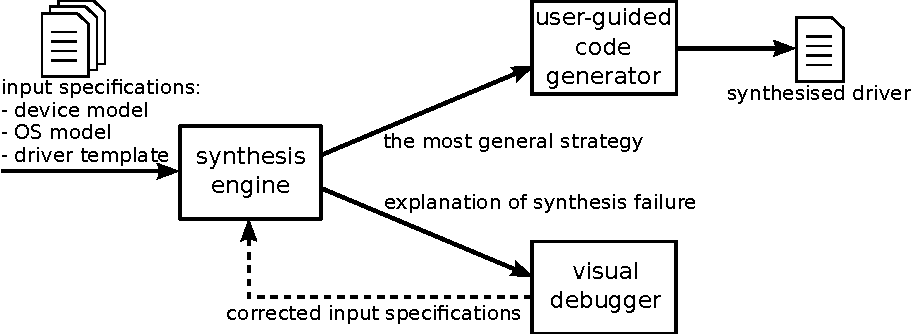
\includegraphics[width=\linewidth]{diagrams/termite.pdf}
    \caption{\termite synthesis workflow.}\label{f:termite}
\end{figure}

Given these specifications, driver synthesis proceeds in two steps.  The first step is carried out fully automatically by the \termite game-based synthesis engine, which computes \emph{the most general strategy} for the driver---a data structure that compactly represents all possible correct driver implementations.  This step encapsulates the computationally expensive part of synthesis.  At the second step, the most general strategy is used by the \termite code generator to construct one specific driver implementation in C with the help of interactive input from the user.

The synthesis engine may establish that, due to a defect in one of the input specifications, there does not exist a specification-compliant driver implementation.  In this case, it produces an explanation of the failure, which can be analysed with the help of the \termite debugger tool in order identify and correct the defect.

%        order to help the developer identify and correct the 
%        defect, the synthesis engine generates a data structure, 
%        called \emph{counterexample strategy}, representing device 
%        and OS behaviour that exposes the defect.  The driver 
%        developer uses the \termite visual debugger tool 
%        (Section~\ref{}) to explore the counterexample strategy, 
%        identify and correct the defect.  
        
%    \item We present the design an implementation of \termite in 
%    a top-down fashion.  We first explore the tool from the 
%    user's perspective.  
%
%        how input specifications for driver synthesis are created
%        
%        next, we explain how the user interacts with the \termite 
%        code generator to produce a well structured driver 
%        implementation.
%        
%        Next we look under the hood

\subsection{Limitations of \termite}  The device driver synthesis technology is still in its early days and, as such, has several important limitations.  Most notably, \termite does not currently support synthesis or verification of code for managing direct memory access (DMA) queues.  This code must be written manually and is treated by \termite as an external API invoked by the driver.  As another example, in certain situations, explained in Section~\ref{s:user-guided}, \termite is unable to produce correct code without user assistance; however it is able to verify the correctness of user-provided code.  We discuss limitations of \termite in more detail in Section~\ref{s:limitations}.

\section{Specifications}

\label{s:specifications}

Input to \termite consists of the three specifications, which model the complete system consisting of the driver, the device, and the OS, shown in Figure~\ref{f:actions}.  The OS and device models simulate the execution environment of the driver and specify constraints on correct driver behavior.  The device model simulates software-visible device behavior.  The OS model serves as a workload generator that issues I/O requests to the driver and accepts request completions in a way consistent with real OS behavior.

\begin{figure}
    \center
    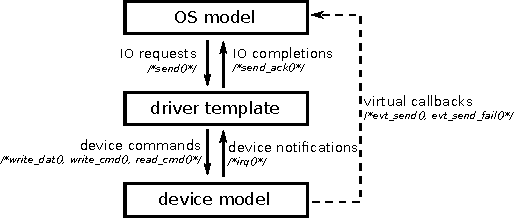
\includegraphics[width=0.85\linewidth]{diagrams/actions.pdf}
    \caption{Input specifications for driver synthesis.  
    Labels in italics show interfaces from the running example
    (Figure~\ref{f:ex}).}\label{f:actions}
\end{figure}

The virtual interface between the device and the OS, shown with the dashed arrow in Figure~\ref{f:actions}, is used by the device model to notify the OS model about important hardware events, such as completion of I/O transactions and error conditions.  Methods of the virtual interface do not represent real runtime interactions between the device and the OS, but are used by the OS model to specify correctness constraints for the driver (see Section~\ref{s:virt}).

Finally, the driver template contains a partial driver implementation to be completed by \termite.  A minimal template consists of a list of driver entrypoints without implementation.  At the other extreme, it can provide a complete implementation, in which case \termite acts as a static verifier for the driver.

All specifications are written using the \termite Specification Language (\tsl).  In line with our goal of making synthesis as close to the conventional driver development workflow as possible, \tsl is designed as a dialect of C with additional constructs for use in synthesis.  We introduce relevant features of \tsl throughout this section.

We minimize the amount of work needed to develop specifications for every synthesized driver by maximizing the reuse of specifications.  In particular, \termite allows the use of existing device specifications developed by hardware designers in driver synthesis.  Furthermore, the OS specification for the driver can be derived from a generic specification for a class of similar devices (e.g., network or storage).  Thus we expect that additional per-driver effort will consist of: (1) inserting device-class callbacks in appropriate locations of the device model and (2) extending the OS specification to support device-specific features missing in the  generic OS specification.

\subsection{Device model}

The device model simulates the device operation at a level of detail sufficient to synthesize a correct driver for it.  To this end, it must accurately model external device behavior visible to software.  At the same time, it is not required to precisely capture internal device operation and timing, as these aspects are opaque to the driver.

Such device models are routinely developed by hardware designers for the purposes of design exploration, simulation, and testing. They are widely used by hardware manufacturers in-house~\cite{cofluent} and are available commercially from major silicon IP vendors~\cite{vp}.  These models are known as \emph{transaction-level models} (TLMs) (in contrast to the detailed register-transfer-level models used in gate-level synthesis)~\cite{Cai_Gajski_03}.  A TLM focuses on software-visible events, or \emph{transactions}, such as a write to a device register or a network packet transmission.

%\change{While the transaction-level modeling technology is 
%relatively new, TLMs are already widely used by hardware 
%manufacturers in-house~\cite{cofluent} and are available 
%commercially from major silicon IP vendors~\cite{vp}.  We expect 
%that in the future open-source TLMs will become commonplace, since 
%a TLM does not expose internal implementation details of the 
%device and is therefore not part of sensitive IP.}

%In the actual hardware circuit a transaction can take multiple 
%(possibly thousands) clock cycles.

%(it does not have a receive function).

\begin{figure}
\lstset{numbers=left}
\lstset{firstnumber=last}
    \scriptsize
%\begin{tabular}{p{0.45\textwidth}p{0.05\textwidth}p{0.45\textwidth}}
%            \center
\begin{tsllisting}[name=ex]
template dev /* Device model */
  uint8 reg_dat, reg_cmd, reg_status = 0;
  /* device commands */
  controllable void write_dat(uint8 v) 
  { reg_dat = v; };
  controllable void write_cmd(uint8 v) 
  { reg_cmd = v; };
  controllable uint8 read_cmd() 
  { return reg_cmd; };
  controllable uint8 read_status() 
  { return reg_status; };
  /* internal behavior */
  process ptx {
    forever {
      wait (reg_cmd == 1);
      choice {
        { os.evt_send(reg_dat);
          reg_status=0; };
        { os.evt_send_fail(reg_dat);
          reg_status=1; };
      };
      reg_cmd = 0;
      /*drv.irq(); (see Section 4*/
    };
  };
endtemplate

template os /* OS model */
  uint8 dat;
  bool inprogress, acked, success;
  /* driver workload generator */
  process psend {
    forever {
      dat = *; /*randomise dat*/
      inprogress = true;
      acked = false;
      drv.send(dat);
      wait(acked);
    };
  };
  /* I/O completions */
  controllable void send_ack(bool status) {
    assert (!inprogress && !acked && 
            status == success);
    acked = true;
  };
  /* virtual callbacks */
  void evt_send(uint8 v) {
    assert (inprogress && v==dat);
    inprogress = false;
    success = true;
  };
  void evt_send_fail(uint8 v) {
    assert (inprogress && v==dat);
    inprogress = false;
    success = false;
  };
  goal idle_goal = acked;
endtemplate

template drv /* Driver template */
  void send(uint8 v){...;};
  /*void irq(){...;}; (see Section 4)*/
endtemplate
\end{tsllisting}
    \caption{\small Trivial serial controller driver specifications.}
    \label{f:ex}
\end{figure}

Existing TLMs created by hardware designers can be used with minor modifications (explained in Section~\ref{s:virt}) for driver synthesis.  Model reuse dramatically reduces the effort involved in synthesizing a driver and is therefore crucial to practical success of driver synthesis.  By reusing an existing model, we also reuse the effort invested by hardware designers into testing and debugging the model throughout the hardware design cycle, thus making driver synthesis less susceptible to specification bugs.  Finally, since TLMs are created early in the hardware design cycle, TLM-based driver synthesis can be carried out early as well, thus removing driver development from the critical path to product delivery.

TLMs are written in high-level hardware description languages like SystemC and DML.  In order to use these models in driver synthesis, we need to convert them to \tsl.  This translation can be performed automatically, and we are currently working on a DML-to-\tsl compiler.  Since this work is not yet complete, device models used in the experimental section of this paper are either manually translated from existing TLMs or written from scratch using TLM modeling style guidelines~\cite{dml_ug}.

%Unfortunately, few TLMs are publicly available at the moment, 
%which means that driver synthesis must be performed by  device 
%vendors in-house.  However this is likely to change in the future.  
%A TLM does not expose internal implementation details of the 
%device and is therefore not part of sensitive IP.  At the same 
%time, there exist strong incentives for manufacturers to make 
%device TLMs available to third-party vendors to test their 
%software and hardware products for compatibility with the given 
%device.

\subsubsection{Running example}

The top part of Figure~\ref{f:ex} shows a fragment of a model of a trivial serial controller device used as a running example.  The fragment specifies the send logic of the controller, which allows software to send data characters over the serial line.  The model is implemented as a \tsl \emph{template}.  The template encapsulates data and code that manipulates the data, similar to a class in OOP.

The software interface of the device consists of data, command, and status registers declared in line~2.  The registers can be accessed from software via the \src{write\_dat}, \src{write\_cmd}, \src{read\_cmd}, and \src{read\_status} methods (lines~4--11).  The \src{controllable} qualifier denotes a method that is available to the driver and can be invoked from synthesized code.

The transmitter logic is modelled in lines~13--25.  It is implemented as a \tsl \emph{process}.  A \tsl specification can contain multiple processes.  The choice of the process to run is made non-deterministically by the scheduler.  The process executes atomically until reaching a \src{wait} statement or a controllable placeholder (see below).

In line~15, the transmitter waits for a command, issued by the driver by writing value $1$ to the command register.  Upon receiving the command, it sends the value in the data register over the serial line.  The transmission may fail, e.g., due to a serial link problem.  The device signals transmission status to software by setting the status register to $0$ or $1$.  Finally, it clears the command register, thus notifying the driver the request has completed.

Internally, the transmitter circuit consists of a shift register and a baud rate generator used to output data on the serial line.  These details are not visible to software and are abstracted away in the model.  We use the non-deterministic \src{choice} construct to choose between successful transmission and failure, without modelling the details of serial link operation.  Successful and failed transmissions are modelled using\src{evt\_send} and \src{evt\_send\_fail} events, explained in Section~\ref{s:os}.

%The \src{ptx} process is initially paused in line~15.  Upon 
%observing value $1$ written to the command register, it sends the 
%value in the data register over the serial line.  The transmission 
%may fail, e.g., due to a serial link problem.  This behavior is 
%modelled using the \src{choice} construct in line~16, which 
%non-deterministically chooses between successful transmission and 
%failure.  The two outcomes are modeled by the \src{evt\_send} and 
%\src{evt\_send\_fail} events respectively.  The device sets the 
%status register to $0$ or $1$ to reflect the 
%
%The actual implementation of the transmitter circuit contains much 
%more detail than captured by this specification.  

\subsection{OS model}\label{s:os}

The OS model specifies the API mandated by the OS for all drivers of the given type.  For example, any Ethernet driver must implement the interface for sending and receiving Ethernet packets.  A separate specification is needed for each supported OS, as different OSs define different interfaces for device drivers.

%A high degree of specification reuse can be achieved by  creating 
%a library of generic specifications for common types of drivers, 
%e.g., network, storage, or serial drivers.  A generic 
%specification describes the API mandated by the OS for all drivers 
%of the given type.  For example, any Ethernet driver must 
%implement the interface for sending and receiving Ethernet 
%packets.  A separate generic specification is needed for each 
%supported OS, as different OSs define different interfaces for 
%device drivers.

Additionally, each particular device can support non-standard features, e.g., device-specific configuration options or transfer modes.  These features must be added as extensions to the generic OS specification in order to synthesize support for them in the driver.  \tsl supports such extensions in a systematic way via the template inheritance mechanism.  We do not describe this in detail due to limited space.

\subsubsection{Running example}

The OS model is written in the form of a test harness that simulates all possible sequences of driver invocations issued by the OS.  The \src{os} template in Figure~\ref{f:ex} shows the OS model for our running example.  The main part of the model is the \src{psend} process.  At every iteration of the loop, it non-deterministically chooses an 8-bit value (line~34) and calls the \src{send} method of the driver, passing this value as an argument.  It then waits for the driver to acknowledge the transmission of the byte (line~38) before issuing another request.  The driver acknowledges the transmission via the \src{send\_ack} callback (line~42).  The callback sets the \src{acked} flag, which unblocks the \src{psend} process.

We keep the specification concise by modeling the state of the driver-OS interface, as opposed to the internal OS state and behavior.  For example, the \src{acked} variable (line~30) serves to model the flow of data between the OS and the driver and is not necessarily present in the OS implementation.

%As another example, we use non-determinism in line~26 to model all 
%possible data values passed to the driver while abstracting away 
%the data path from a user-level program to the driver via various 
%kernel subsystems.

\subsection{Connecting device and OS models}\label{s:virt}

In addition to simulating I/O requests to the driver, the OS model also specifies the semantics of each request in terms of device-internal events that must occur in order to complete the requested I/O operation.  In our running example, after the OS invokes the \src{send} method of the driver and before the driver acknowledges completion of the request, the device must attempt to send the requested data over the serial line.  This requirement establishes a connection between the device and OS models and must be specified explicitly in order to enable \termite to generate a driver implementation that correctly handles the OS request.  Note that we only need to specify \emph{which} hardware events must occur, but not \emph{how} the driver generates them.

In order to develop such specifications, we need a way to refer to relevant state and behavior of the device from the OS model.  At the same time, in order to maximize specification reuse, we would like to keep the OS specification device-independent.  To reconcile these conflicting requirements, we introduce a \emph{virtual interface} between the device and OS model.  This interface consists of callbacks used by the device model to notify the OS model about important hardware events.  The virtual interface does not represent real runtime interactions between the device and the OS, but serves as part of the correctness specification.

We define a virtual interface for each class of devices.  Such \emph{device-class} interfaces are both device and OS-independent.  The device-class interface can be extended with additional device-specific callbacks as required to specify a driver for a particular device.

\subsubsection{Running example}

In our example, we define a device-class interface consisting of two virtual callbacks: \src{evt\_send} and \src{ev\_send\_failed}, invoked respectively when the device successfully transmits and fails to transmit a byte.  These callbacks are invoked in lines~17 and 19 of the device model.  The \src{evt\_send} handler is shown in line~48 of the OS model.  The assertion in line~49 specifies that the send event is only allowed to occur if there is an outstanding send request in progress and the value being sent is the same as the one requested by the OS.  We reset the \src{inprogress} flag to false in line~50, thus marking the current request as completed; line~51 sets the \src{success} flag to true, thus indicating that the transfer completed without an error.  The \src{evt\_send\_fail} handler is identical, except that it sets the \src{success} flag to false.  The flags are checked by the \src{send\_ack} method, which asserts that the driver is only allowed to acknowledge a completed request (\src{!inprogress}) that has not been acknowledged yet (\src{!acked}) and that the completion status reported by the driver must match the one recorded in the \src{success} flag.

In this example we use C-style assertions to rule out invalid system behaviors.  Assertions alone do not fully capture requirements for a correct driver behavior.  For example, a driver that remains idle does not violate any assertions.  Hence, we need to specify requirements for the driver to make forward progress.  We introduce such requirements into the model in the form of \emph{goal conditions}, that must hold \emph{infinitely often} in any run of the system.  For example, a goal may require that the driver is infinitely often in an idle state with no outstanding requests from the OS.  The OS can force the driver out of the goal by issuing a new I/O request.  To satisfy the goal condition, the driver must return to the goal state by completing the request.  Line~58 in Figure~\ref{f:ex} defines such a goal condition that holds whenever the \src{acked} flag is set, i.e., the driver has no unacknowledged send requests.

\subsection{Driver template}

The bottom part of Figure~\ref{f:ex} shows the driver template for the running example consisting of a single \src{send} entry point invoked by the OS.  The ellipsis in line~62 represent a location for inserting synthesized code and are part of \tsl syntax.  We refer to such locations as \emph{controllable placeholders}. 

\section{Heuristic code generation}

\section{User-guided code generation}
\label{s:user-guided}

The set of input \tsl specifications is fed into the \termite synthesis engine, which then automatically computes the most general strategy for the driver.  Given a state of the system, the most general strategy determines the set of all valid driver actions in this state.  The most general strategy is used by the \termite code generator to produce a driver implementation in C in a user-guide fashion.


%\paragraph{Experience with automatic code generation}
%
%Early versions of \termite implemented fully automatic code  
%generation as their only mode of operation.  In many cases we 
%found that the tool produced unsatisfactory code
%, which led to a series of improvements to the code generation 
%algorithm, aimed to generate more compact, user-readable, and 
%efficient implementations.  At the same time, we found that many 
%aspects of what is perceived by developers as a good 
%implementation are very hard to formalize, and, even when 
%possible, the effort involved in such a formalization exceeds the 
%effort needed to achieve the desired effect manually.
%
%For example, the interrupt handler logic of most drivers follows
%the standard structure, where the driver checks every interrupt
%source in the order of its priority and invokes a separate handler
%function for every signaled interrupt.  Interrupt prioritization
%and functional decomposition are hard to synthesize automatically
%without manual guidance.
%
%One might argue that structure and readability are not relevant
%for synthesized code.  In practice, however, if synthesized
%drivers are to make their way into Linux and other major OSs, they
%must follow standard coding guidelines adopted by these OSs and be
%amenable to manual code inspection.  Furthermore, human readable
%code is needed for quality assurance.  While automatic synthesis
%guarantees that the synthesized driver is correct with respect to
%input specifications, it does not protect against specification
%defects: despite our best effort to maximize specification reuse
%and follow good modeling practices, specification defects cannot
%be avoided altogether.  Hence, manual inspection remains an
%important way to eliminate driver bugs.
%
%In summary, while there exists a potential for further improvement
%of automatic code generation algorithms, we believe that a truly
%practical driver synthesis tool must put the user in control of
%the resulting code and not enforce any particular code structure
%nor attempt to override user's design decisions.
%
%\paragraph{User-guided code generation}

%The code generator works as advanced auto-complete, that can be 
%used to generate a single statement or an entire function.  
%\termite automatically and on the fly verifies that the driver 
%implementation, comprised of a mix of generated and manually 
%written code, is consistent with the most general strategy, thus 
%maintaining strong correctness guarantees that one would expect in 
%automatically synthesized code.

The \termite code generator GUI is similar to a traditional integrated development environment with two additional built-in tools: the \emph{generator} and the \emph{verifier}.  The generator works as advanced auto-complete that helps the user to fill the controllable placeholders inside the driver template with code.  At any point, the user can invoke the generator to synthesize a single statement or a complete block of code inside a controllable placeholder via a mouse click on the target code location.  The user can arbitrarily modify and amend the generated code.  However, the generator never modifies user code.  Instead it tries to extend it to a complete implementation, which is always possible provided that the existing code is consistent with the most general strategy.  The generator currently only allows synthesizing statements after the last control location within a branch.  However this restriction is not a conceptual one and will be lifted by ongoing development.

The verifier automatically and on the fly checks that the driver implementation, comprised of a mix of generated and manually written code, is consistent with the most general strategy, thus maintaining strong correctness guarantees that one would expect in automatically synthesized code.  The verifier symbolically simulates execution of the system, following the partial driver implementation created so far, and signals the user whenever it encounters a transition that violates the most general strategy.

In the first approximation, the generator algorithm is quite simple: given a source code location, it determines the set of possible system states in this location, picks an action for each state from the most general strategy and translates this action into a code statement.  In practice the algorithm uses a number of heuristics to produce compact and human-readable code.  In particular, whenever there exists a common action in all possible states in the given location, the algorithm produces straight-line code without branching.  For example, when running the generator on the specification in Figure~\ref{f:ex}, it automatically generates the following code for the \src{send} function(line~62):

\begin{tsllisting}[keywords=, frame=single]
void send(uint8 v){
    dev.write_dat(v);
    dev.write_cmd(1);
    wait(dev.reg_cmd==0);
    if (os.success) {
        os.send_ack(true);
    } else {
        os.send_ack(false);
    };}
\end{tsllisting}

This implementation correctly starts the data transfer by writing the value to be sent to the data register and setting the command register to $1$.  It then waits for the transfer to complete, which is signalled by the device by resetting the command register to $0$.  Finally, it acknowledges the completion of the transfer to the OS.

Note that the generated code refers to the \src{dev.reg\_cmd} and \src{os.success} variables.  These variables model internal device and OS state respectively and cannot be directly accessed by the driver.  This example illustrates an important limitation of \termite---it assumes a white-box model of the system, where every state variable is visible to the driver.  Ideally, we would like to synthesize an implementation that automatically infers the values of important unobservable variables.  In this case, the value of the command register can be obtained by the driver by executing the \src{read\_cmd} action.  Furthermore, the value of the \src{os.success} variable is correlated with the completion status of the last transfer, which can be obtained by reading the device status register.

While \termite currently cannot produce such an implementation automatically, it implements a pragmatic tradeoff that helps the user build and validate a correct implementation with modest manual effort.  The code generator warns the user that the auto-generated code accesses  private variables of the device and OS templates.  This prompts the user to provide a functionally equivalent valid implementation, replacing the \src{wait} statement with a polling loop and using the \src{read\_status} method to check transfer status:

\begin{tsllisting}[keywords=, frame=single]
void send(uint8 v){
    dev.write_dat(v);
    dev.write_cmd(1);
    (*@{\bf\ttfamily while(dev.read\_cmd()==1){};}@*)
    if ((*@\bf\ttfamily dev.read\_status()@*)) {
        os.send_ack(true);
    } else {
        os.send_ack(false);
    };}
\end{tsllisting}

The verifier automatically checks the resulting implementation and confirms that it satisfies the input specification.

Note that in this example we have synthesized code that correctly handles device errors.  This was possible, as our input device specification correctly captures device failure modes (namely, transmission failure) and our OS specification describes how the driver must report errors to the OS (via the \src{status} argument of the completion callback).

In principle, it is also possible to synthesize a driver implementation that handles device and OS failures \emph{not} captured in the specifications: since the synthesis tool knows all possible valid environment behaviors, it can easily detect invalid behaviors and handle them gracefully.  Automatic synthesis of such \emph{hardened} device drivers is a promising direction of future research.

The final step of the code generation process translates the synthesized driver implementation to C.  This is a trivial line-by-line translation.  We expect this translation to become unnecessary in the future as our ongoing work on the \tsl syntax aims to make the synthesized subset of \tsl a strict subset of C.

\subsection{Maintaining synthesized code~~} 
Device driver development is not a one-off task: following the initial implementation, drivers are routinely modified toimplement additional functionality, adapt to the changing OS interface or support new device features.

The user-guided code generation method naturally supports such incremental maintenance. Since \termite uses \tsl as both its input and output language;  a completely or partially synthesized driver can be given as input to \termite, along with modified versions of the device and OS models.

A typical maintenance task proceeds in three steps.  First, the developer amends device and OS models to reflect the new or changed functionality.  Second, they add new methods to the previously synthesized driver, if necessary, and replace existing driver code that is expected to change with a controllable  placeholder.  Finally, the user runs \termite to synthesize code for all controllable placeholders.  \termite treats all existing driver code as part of the uncontrollable environment.  Hence, if some of the old code is incorrect in the context of the new specifications, this will lead to a synthesis failure, and counterexample-based debugging is used to identify the faulty code, as described in Section~\ref{s:debug}.

As an example, we synthesize a new version of the driver for our running example assuming a more advanced version of the serial controller device that uses interrupts to notify the driver on completion of a data transfer.  The new device model is obtained by uncommenting line~23 of the device model in Figure~\ref{f:ex}, which invokes the interrupt handler method of the driver after each transfer.  The driver template is extended with the \src{irq} method (line~63).  We use the previously synthesized implementation of the \src{send} method, but manually remove the last two lines, which implement polling, as we want the new implementation to use interrupts instead:

\begin{tsllisting}[keywords=, frame=single]
void send(uint8 v){
    dev.write_dat(v);
    dev.write_cmd(1);}
\end{tsllisting}

Finally, we run \termite on the resulting specifications and use the generator to automatically produce the following implementation of the new \src{irq} method:

\begin{tsllisting}[keywords=, frame=single]
void irq(){
    if (os.success) {
        os.send_ack(true);
    } else {
        os.send_ack(false);
    };}
\end{tsllisting}

As before, we manually replace the if-condition in the first line with

\begin{tsllisting}[keywords=, frame=single]
if (dev.read_status())
\end{tsllisting}

This example illustrates how \termite supports incremental changes to the driver by reusing previously synthesized code, while maintaining strong correctness guarantees.

\subsection{Instrumenting synthesized code~~} 
\termite does not automatically instrument synthesized code for debugging, logging, accounting, etc.  However, the user can add such instrumentation manually.  \termite interprets such code as no-ops and, as with any manual code, never makes any modifications to it.

\section{Counterexample guided debugging}

An important practical issue in game-based synthesis is the complexity of diagnosing synthesis failures due to defects in the input specifications.  In the event that \termite fails to solve the game, the user needs to trace the failure back to the specification defect.  However, the failure does not carry any information about the defect, which makes the problem harder to resolve.

In \termite we propose a new approach to troubleshooting synthesis failures based on the use of \emph{counterexample strategies}.  A counterexample strategy is a strategy on behalf of the environment that prevents the driver from winning the game.  It is obtained by solving the \emph{dual game}, where, in order to win, the environment must permanently force the game out of one of the goal regions.  A winning strategy in the dual game is guaranteed to exist whenever solving of the primary game fails.

%    \item By exploring the counterexample strategy, the user can 
%        identify the defect in the input specification.  This is 
%        similar to the use of counterexamples in software 
%        verification, where for each discovered bug the 
%        verification tool generates a counterexample trace that 
%        triggers the bug.  However, a counterexample strategy 
%        cannot in the general case be represented by a single 
%        execution trace, as the choice of spoiling moves for the 
%        environment depends on the actions performed by the 
%        driver.

In order to detect and fix the defect in an input specification, the driver developer relies on their  understanding of the OS and device logic.  The role of the counterexample strategy is to guide the developer towards the defect.  To automate this process, we developed a powerful visual debugging tool that allows the user to interactively simulate intended driver behavior and observe environment responses to it.  The user plays the game on behalf of the driver, while the tool responds on behalf of the environment, according to the counterexample strategy.
 
In a typical debugging session, the debugger, following the counterexample strategy, generates a sequence of requests that are guaranteed to win against the driver.  The user plays against these requests by specifying device commands that, they believe, represent a correct way to handle the request.  Since this sequence of requests \emph{cannot} be handled correctly given the current input specification, at some point in the game the user runs into an unexpected behavior of one of the players, e.g., one of user-provided commands does not change the state of the device as expected or the environment performs an uncontrollable transition that violates an assertion.  Based on this information, the user can revise the faulty specification.

%       
%        To this end, we developed a powerful visual debugging tool 
%        that allows the user to interactively simulate intended 
%        driver behaviour and observe enviroment responses to it.  
%        The user plays the game on behalf of the driver, while the 
%        tool responds on behalf of the enviroment 
%        
%        We rely on the fact that the driver developer has a good 
%        understanding of the OS and device logic.  Given that 
%        there does not exist a specification-compliant driver 
%        implementation, our goal is to help the developer to 
%        identify a discrepancy between their mental model of the 
%        system behaviour and the acual behaviour as described in 
%        the input specifications.  To this end, we developed a 
%        powerful visual debugging tool that allows the user to 
%        interactively simulate intended driver behaviour and 
%        observe enviroment responses to it.  The user plays the 
%        game on behalf of the driver, while the tool responds on 
%        behalf of the enviroment.

At every step of the interactive debugging session, the debugger either chooses a spoiling uncontrollable action based on the counterexample strategy or, if the system is inside a controllable placeholder, allows the user to choose a controllable action to execute on behalf of the driver.  In the former case the spoiling uncontrollable action corresponds to a transition in one of the \tsl processes.  The user can explore this transition by stepping through it, exactly as they would in a conventional debugger.  In the latter case, the user provides the action that they would like to perform by typing and executing corresponding code statements.

The tool supports a number of features aimed to make the debugging process as simple as possible for the user. We mention two of them here.  First, the debugger interactively prompts actions available to the driver at each step.  Second, the debugger keeps the entire history of the game and allows the user to go back to one of previously explored states and try a different behavior from there.

\section{Limitations}\label{s:limitations}

In Section~\ref{s:user-guided}, we described one limitation of \termite, namely the lack of support for grey-box synthesis.  In this section we discuss other limitations, which, we hope, will help define the agenda for continuing research in driver synthesis.

%The core of a device driver entails translating I/O requests from 
%the OS into sequences of low-level device commands and responses.  
%We focus on synthesizing driver logic that performs these 
%functions, and this is where game-based synthesis really shines, 
%as it helps to implement tedious and error-prone logic with 
%minimal manual effort and without bugs.


%The other important limitation of \termite is that its game-based 
%synthesis engine currently assumes the white-box view of the 
%system, where the driver can fully observe the state of the 
%system, including internal device state.  As a result, 
%automatically synthesized driver code may refer to state variables 
%outside of its syntactic scope.  As we explain in 
%Section~\ref{s:user-guided}, our user-guided synthesis approach 
%resolve such situations by relying on manual user input.

\subsection{Direct Memory Access}

Most importantly, \termite does not currently support automatic synthesis of direct memory access (DMA) management code.  Many modern devices transfer data directly to and from main memory, where it is buffered in data structures such as circular buffers and linked lists.  These data structures can have very large or infinite state spaces and cannot be easily modeled within the finite state machine-based framework of \termite.  Efficient synthesis for DMA requires enhancing the synthesis algorithm to use a more compact representation of DMA data structures, which is the focus of our ongoing research.  At this time, code for manipulating DMA data structures must be written manually.  This code is not interpreted or verified by \termite.  For example, we use this approach to synthesize a DMA-capable IDE disk driver (Section~\ref{s:eval}).

\subsection{Boilerplate Code}

Device drivers in modern OSs contain a significant amount of boilerplate code that is not directly related to the task of controlling the device.  This includes binding the driver to I/O resources (memory mapped regions, interrupts, timers), registering the driver with various OS subsystems, allocating DMA memory regions, creating sysfs entries, etc.  While much of this functionality could be synthesized within the game-based framework, we do not believe that this is the correct approach.  Previous research has demonstrated that this boilerplate code can be generated in a principled way from declarative specifications of the driver's requirements and capabilities~\cite{Spear_RHHL_06}.  This technique has lower computational complexity than game solving and better captures the essence of the task.  A practical driver synthesis tool cancombine game-based synthesis of the core driver logic responsible for controlling the device with declarative synthesis of boilerplate code.  As a result, the current version of \termite assumes this boilerplate code is written manually as a wrapper around the synthesized driver.

\subsection{Concurrency}

Drivers execute in a concurrent OS environment and must handle invocations from multiple threads, as well as asynchronous hardware interrupts.  We separate synthesis for concurrency into a separate step.  Drivers synthesized by \termite are correct assuming a sequential environment, where driver entry points are invoked atomically.  The resulting sequential driver is then processed by a separate tool that performs a sequence of transformations of the driver source code, which preserve the driver's sequential behavior, while making the driver thread-safe.  Such transformations include adding locks around critical code sections, inserting memory barriers, and reordering instructions to avoid race conditions.  Concurrency synthesis is still work in progress and is beyond the scope of this paper.  Our preliminary results are published in~\cite{Cerny_HRRT_13, Cerny_HRRT_14}.

\subsection{Real time synthesis}

\termite does not explicitly support specification and synthesis of timed behaviors.  Instead, it uses a pragmatic approach that allows it to synthesize time-sensitive behavior without having to explicitly reason about time.  To this end, \termite conservatively approximates timed operations by fairness constraints: it ignores the exact duration of each device operation, but keeps the knowledge that the operation will complete \emph{eventually}, and synthesizes a driver that waits for the completion.  \termite is also able to handle time-out conditions, modeled as external events.  However, at this time it is not capable of generating device drivers for hard real-time systems, where the driver must guarantee completion of I/O operations by a certain deadline.

\section{A realistic example}

\section{Implementation}

We implemented all components of the Termite toolkit, including the TSL compiler, the game solver, the counterexample debugger, the user-guided code generator, and the TSL-to-C compiler, in Haskell.  Our implementation uses the CUDD BDD library for efficient symbolic manipulations over boolen relations, and the Z3 SMT solver for satisfiability queries over the theory of bit vectors, as described in~\cite{Walker_Ryzhyk_14}.  Termite is publicly available under the BSD license and can be downloaded from the project website \texttt{\url{http://termite2.org}}. The version of \termite presented here consists of 30,000 lines of code.  The estimated overall project effort is 10 person years. 

\section{Evaluation}
We evaluate \termite by synthesizing drivers for eight I/O devices.  Specifically, we synthesized drivers for a UVC-compliant USB webcam, the 16550 UART serial controller, the DS12887 real-time clock, and the IDE disk controller for Linux, as well as seL4~\cite{Klein_EHACDEEKNSTW_09} drivers for I2C, SPI, and UART controllers on the Samsung exynos 5 chipset\footnote{At the time of writing, the exynos drivers have not yet been tested due to hardware availability issues; however we confirmed via manual inspection that they implement the same device control sequences as existing manually developed drivers.} and SPI controller on the STM32F10 chipset.  With the exception of the IDE disk, these devices are representative of peripherals found in a typical embedded platform, such as a smartphone.  Our synthesized drivers implement data transfer, configuration and error handling.  The main barrier to synthesizing drivers for more advanced devices, e.g., high-performance network controllers, is the current lack of support for synthesis of DMA code in the current version of \termite.  

\subsection{Modelling complexity} 
Models of UART and DS12887 devices were developed based on existing publicly available device models~\cite{ds12887, uart}.  Models of other devices were derived from their vendor-provided documentation, following standard TLM modeling guidelines~\cite{dml_ug}.  OS models for the relevant device classes were created based on Linux kernel documentation and source code.  

Table~\ref{t:size} summarises the size, in lines of code, of device and OS models in our case studies.  Developing a complete set of specifications for each driver took approximately one week, of which only one to three days were spent building the models and the rest of the time was spent studying device and OS documentation.  This efficiency can be attributed to the choice of the right level of abstraction and modeling language.  In particular, the use of transaction-level device modeling abstracts away complicated internal device machinery by focusing on high-level events relevant to driver synthesis, while the \tsl language allows modeling the driver environment using standard programming techniques, as illustrated by our running example.

\begin{table}
    \begin{minipage}{\linewidth}
    \center
    %\begin{tabular}{|p{0.15\linewidth}|p{0.15\linewidth}p{0.15\linewidth}|p{0.15\linewidth}p{0.15\linewidth}|}
    \begin{tabular}{|l|c|c|c|c|}
        \hline
%        & \multicolumn{4}{|c|}{size (lines of code)} \\
%        \cline{2-5}
        & \multicolumn{2}{|c|}{input spec} & \multicolumn{2}{c|}{driver} \\
        \cline{2-5}
                     & OS  & device & synthesized & native \\
        \hline
        \hline
        webcam       & 102 & 385    & 113         & 307 \\
        16450 UART   & 122 & 167    & 74          & 261 \\
        exynos UART  & 128 & 252    & 37          & 166 \\
        STM SPI      & 73  & 244    & 24          & 64  \\
        exynos SPI   & 88  & 239    & 40          & 183 \\
        exynos I2C   & 146 & 180    & 79          & 211 \\
        RT clock     & 118 & 252    & 84          & 183 \\
        IDE          & 188 & 480    & 94\footnote{Excluding 36 lines of manually written code that manipulates the DMA descriptor table.} & 474 \\
        \hline
    \end{tabular}
    \end{minipage}
    \caption{Size (in lines of code) of input specifications and of synthesized and equivalent manually written drivers.}
    \label{t:size}
\end{table}

Interestingly, we found the most error-prone step in developing specifications for driver synthesis to be defining correct relative ordering of OS-level and device-level events with the help of the virtual interface (Section~\ref{s:virt}).  Na\"ive specifications tend to be either too restrictive, leading to synthesis failures, or too liberal, leading to incorrect synthesized drivers. As we gained more experience synthesizing different types of drivers, we identified common modeling patterns that help avoid errors in virtual interface specifications.  

As a common example, most virtual interfaces contain callbacks that signal a change to one of device configuration parameters, e.g., transfer speed, parity, etc.  A na\"ive OS model may only allow such a callback to be triggered when the OS has requested a change to the corresponding device setting.  However, many devices only allow setting multiple configuration parameters simultaneously, so that setting any individual parameter triggers multiple callbacks, thus making the specification non-synthesizable.  The problem can be rectified by changing the device specification to only trigger callbacks if the new value of the parameter is different from the old one; however this bloats the device model due to the extra checks.  A better solution, used in all our models, is to design the OS specification to allow configuration callbacks to be triggered at any time, provided that the new value of the parameter is equal to the last value requested by the OS. 

\subsection{Synthesis time} 
Table~\ref{t:perf} summarises the performance of the \termite game solver in our case studies.  The second column of the table characterises the complexity of the two-player game constructed by the \tsl compiler from the input specifications in terms of the number of states variables and the total number of bits in these variables.  The third column shows the number of iterations of the abstraction refinement loop required to solve the game.  The next column shows the size of the abstract game at the final iteration, in terms of the number of predicates in the abstract state space of the game.  These results demonstrate the dramatic reduction of the problem dimension achieved by our abstraction refinement method.  The second-last column shows that the \termite game solver was able to find the most general winning strategy within a few minutes in all case studies.

\begin{table}
    \center
    \begin{tabular}{|l|ccccc|}
        \hline
                       & \multirow{2}{*}{vars(bits)} & refine- & predi- & synt.     & verif.   \\
                       &                             & ments   & cates  & time (s)  & time (s) \\
        \hline
        \hline
        webcam         & 128 (125565)                & 47      & 192    & 215       & 794 \\
        16450 UART     & 81  (407)                   & 65      & 128    & 210       & 464 \\
        exynos UART    & 80  (1185)                  & 54      & 111    & 645       & 82 \\
        STM SPI        & 68  (389)                   & 29      & 63     & 67        & 31 \\
        exynos SPI     & 83  (933)                   & 31      & 72     & 25        & 44 \\
        exynos I2C     & 65  (303)                   & 21      & 56     & 45        & 96 \\
        RT clock       & 92  (810)                   & 25      & 74     & 56        & 127 \\
        IDE            & 114 (1333)                  & 42      & 105    & 285       & 778 \\
        \hline
    \end{tabular}
    \caption{Performance of the \termite game solver.}
    \label{t:perf}
\end{table}

We compared the performance of the \termite game solver against a state-of-the-art abstraction refinement algorithm for games~\cite{Alfaro_Roy_07} as well as against the standard symbolic algorithm for solving games without abstraction~\cite{Piterman_PS_06}.  In all case studies, the \termite solver was the only one to find a winning strategy within a two-hour limit.  We refer the reader to~\cite{Walker_Ryzhyk_14} for a more detailed performance analysis of the \termite synthesis algorithm.

The final column of Table~\ref{t:perf} shows the time that it took \termite to verify a complete driver.  Recall that the \termite synthesis algorithm doubles as a verification algorithm and can be used to verify drivers written in \tsl.  We used complete synthesized drivers, containing a combination of manual and automatically generated code, as inputs to \termite.  We have been able to successfully verify all of our drivers.  We also experimented with introducing faults to synthesized drivers.  \termite was able to detect these faults and produce correct counterexample strategies.  In most cases verification took longer than synthesis.  The reason for this is that \termite has not yet been optimized for verification workloads.  This is one area for future improvement.

%\termite is the first synthesis tool based on abstraction 
%refinement, so we cannot compare it against other 
%abstraction-based algorithms.  We benchmark \termite against a 
%highly optimized implementation of the state of the art algorithm 
%for solving GR-1 games (without abstraction) by Piterman et 
%al.~\cite{Piterman_PS_06}.  This algorithm was not able to solve 
%any of our case studies within a two-hour time limit.  We 
%therefore produced a simplified version of the IDE case study with 
%only 75 state bits (instead of 1333 in the original 
%specification), which the Piterman et al. algorithm solved in 
%57 minutes.  For comparison, \termite solved this simplified 
%example in under 1 second.

\subsection{User-guided code generation and debugging} 
We evaluate the key contribution of this paper, namely the user-guided debugging and code generation technique.  Each line of code in a \termite-generated driver originates from one of three sources: it can be (1) synthesized automatically by the tool, (2) developed offline and given to \termite as part of the driver template, or (3) added or modified by the user during an interactive code generation session.  A perfect synthesis tool, capable of generating a complete driver fully automatically while producing code that meets all non-functional requirements, would eliminate the need for manual code altogether.  We do not believe that such a tool is feasible in the near future.  We therefore explore the tradeoffs that arise when using our current, imperfect, tool.  In particular, we would like to empirically characterize situations when the user can rely on the synthesizer to automatically produce near-optimal code, and when they are better off completely or partially implementing certain functionality manually.  These tradeoffs are likely to change as the tool improves.

Based on our experience so far, automatic synthesis is most helpful in generating code that performs device configuration or starts a data transfer.  This code may involve a long sequence of commands to the device, which must be issued in the right order and with correct arguments.  The synthesis algorithm of \termite proved more effective at doing this than human developers, producing correct code that only requires minimal cosmetic changes in most cases.  For example, Figure~\ref{f:screenshot_write} shows a screenshot of \termite with a synthesized implementation of the IDE driver \src{write()} function, which starts a data transfer to the device.  The function writes request parameters into appropriate device data registers and sets bit fields in command registers to prepare the device for data transfer.  One deficiency in this auto-generated implementation is that it uses absolute values instead of symbolic constants for bit fields.

As another example of suboptimal synthesized code, consider the following synthesized fragment

\begin{tsllisting}[frame=single]
void packet_received() {
  if (((packet_data[9:9] == 1) && 
       (packet_data[14:14] == 1))) {
    os.ack_packet(1,1,packet_data[16:32]);
  } else if ((dev.packet_data[9:9] == 1)) {
    os.ack_packet(1,0,packet_data);
  } else if ((dev.packet_data[14:14] == 1)) {
    os.ack_packet(0,1,packet_data[16:32]);
  } else {
    os.ack_packet(0,0,packet_data[16:32]);
  };
};
\end{tsllisting}

which can be replaced by an equivalent one-liner

\begin{tsllisting}[frame=single]
os.ack_packet(packet_data[9:9],
    packet_data[14:14],packet_data[16:32]);
\end{tsllisting}

\noindent While both issues can, and will, be addressed by an improved code generation algorithm, our experience shows that unaccounted corner cases will arise occasionally.  Therefore, the ability to manually modify synthesized code without sacrificing correctness is crucial for a practical synthesis tool.

Limitations of \termite are most noticeable in synthesizing interrupt handler code responsible for processing I/O completions.  This involves querying device state to determine which operations completed and with what status, reporting results to the OS, and clearing interrupt status registers.  Since \termite does not support grey-box synthesis, it can not generate this code automatically and instead produces code that directly accesses device-internal state (see Section~\ref{s:user-guided}).  \termite correctly reports such situations and allows the user to mitigate them by manually editing synthesized code.  In practice, however, we found it easier to develop most of the interrupt handler logic offline, as part of the driver template, and rely on \termite to (a) establish correctness of this code and (b) extend it to a complete implementation.

\begin{figure}
    \center
    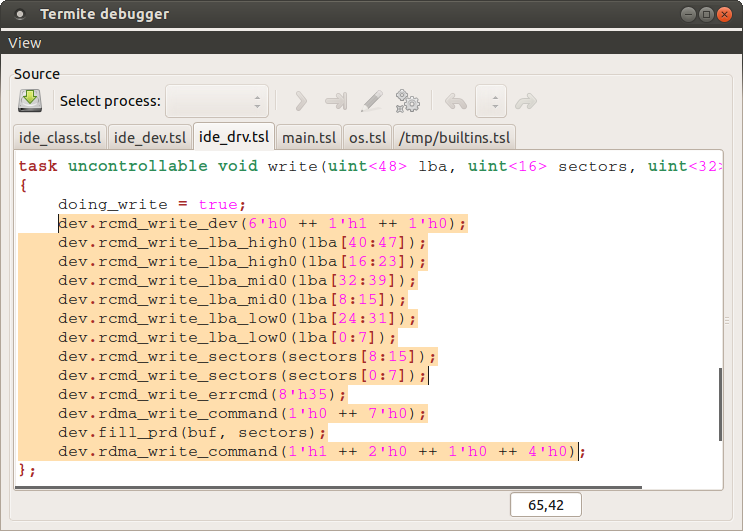
\includegraphics[width=\linewidth]{diagrams/screenshot_write.png}
    \caption{Screenshot of \termite with a synthesized implementation of the IDE driver.  Automatically generated code is highlighted.}
    \label{f:screenshot_write}
\end{figure}

In our case studies, 60\% to 90\% of the code was generated fully automatically, with the rest of the code produced in a user-guided fashion.  Once an initial version of device and OS specifications was ready, it took us several hours to generate the driver implementation for each of our case studies.  Three quarters of this time was spent debugging the input specifications, with the rest of it spent generating driver source code with the help of the user-guided code generation GUI.

We found counterexample-driven debugging to be crucial to the productivity of synthesis-based development.  Before the debugger was available, we had to rely on code inspection to identify defects in the input specifications, which proved to be a frustrating and unpredictably long process.  The \termite debugger streamlines this process, giving us the confidence that any failure can be localised by following well-defined steps.  A typical debugging session takes a few minutes and involves entering only a few commands manually before the defect is localised. 

%We found the incremental approach to debugging and synthesis to 
%be the most effective.  Incremental synthesis 
%
%synthesise a single driver function or a small group of related 
%functions before adding m
%
%This is achieved by disabling invocations of all but one I/O 
%operations in the OS model. 
%
%Incremental synthesis

%In all case studies, we have been able to achieve human-readable 
%code structure that one would expect in a manually developed 
%driver.  60\% to 90\% of the code was generated fully 
%automatically and did not require any manual changes.  The rest of 
%the code was produced in a user-guided fashion, as described in 
%Section~\ref{s:user-guided}.  Human involvement was required for 
%three reasons.  First, it was necessary to get around the 
%white-box assumption, causing automatically generated code to 
%access variables outside the syntactic scope of the driver, as 
%explained in Section~\ref{s:user-guided}.  Second, it was used to 
%enforce a particular preferred implementation among several 
%functionally equivalent alternatives.  A common example of such a 
%situation, illustrated in Section~\ref{s:user-guided}, is 
%implementing I/O completions using interrupts instead of polling.  
%Finally, we relied on manual intervention to improve the structure 
%of synthesized code to make it compliant with the standard Linux 
%driver structure.

\subsection{Size of synthesized code} 
The last two columns of Table~\ref{t:size} compare the size of synthesized drivers to existing manually developed drivers.  Synthesised drivers are significantly more compact than conventional drivers for two main reasons.  First, as explained in Section~\ref{s:limitations}, we only synthesize the driver logic directly responsible for controlling the device.  Conventional drivers typically contain a large amount of boilerplate code managing various OS resources.  We believe that this code can and should be synthesized using complementary techniques.  At the moment we implement this functionality manually as a wrapper around the synthesized driver. 

Second, conventional device drivers are often designed to support multiple similar devices with slightly different interfaces and capabilities.  This leads to code bloat, as the driver must implement multiple versions of various operations, as well as logic to dynamically discover device capabilities and choose the right implementation to use.  In contrast, every \termite driver supports one specific device model with a fixed set of features.  Drivers for similar devices can share common specification code, but are synthesized as separate source code modules.  This approach leads to simpler code and is preferable for platforms with a fixed set of peripheral devices, such as smartphones, where shipping drivers that support only the required devices enables smaller system image.
  
\subsection{Specification reuse}  
Our specification methodology ensures mutual independence of device and OS specifications, and thus facilitates their reuse.  We have not yet carried out a substantial evaluation of such reuse; however we report our limited experience based on synthesizing two SPI drivers for the seL4 OS.  The corresponding OS specification was initially developed during the work on the SPI driver for the exynos chipset.  It was later used to synthesize a driver for the STM32F10 chipset.  We were able to reuse most of the original specification.  Minor changes (8 lines of code) were required in the part of the specification describing configuration functionality of the driver, since the STM SPI controller supports a number of ad hoc transfer modes.  We expect to observe similar pattern for other devices and operating systems: generic OS specifications can be reused with localized, device-specific changes required to support non-standard device features.

\subsection{Performance of synthesized drivers} 
Our synthesized drivers implement effectively identical device control logic to their conventional counterparts and therefore have similar performance.  We benchmarked the USB webcam driver, which is the most performance-critical one among our case studies.  We measured CPU load and data throughput generated by the conventional and synthesized drivers for varying bitrates.  We obtained identical results, modulo measurement errors, for both drivers in all cases.

\chapter{Appendix}

\end{document}
